
\section*{CHƯƠNG 2. PHÂN TÍCH HỆ THỐNG}
\setcounter{section}{2}
\setcounter{subsection}{0} %LƯU Ý MỖI LẦN THÊM CHƯƠNG MỚI CẦN THÊM CÂU NÀY ĐỂ RESET THỨ TỰ CỦA SUBSECTON VỀ 1
\setcounter{table}{0} % LƯU Ý SAU MỖI LẦN GỌI BẢNG HAY HÌNH ẢNH PHẢI THÊM CÂU NÀY ĐỂ RESET THỨ TỰ
\setcounter{figure}{0} %% LƯU Ý SAU MỖI LẦN GỌI BẢNG HAY HÌNH ẢNH PHẢI THÊM CÂU NÀY ĐỂ RESET THỨ TỰ
\addcontentsline{toc}{section}{\numberline{}CHƯƠNG 2. PHÂN TÍCH HỆ THỐNG}
Trong chương này, chúng em sẽ tiến hành phân tích hệ thống cho dự án đề tài "Hệ thống theo dõi và quản lý dữ liệu điện tim" dựa trên các mục tiêu
đã nêu ra trong Mục Đề xuất hệ thống ở Phần mở đầu. Trước tiên bài toán đặt ra ở hệ thống là:
\begin{adjustwidth}{1.5em}{}
\begin{itemize}
  \item Một ứng dụng để có thể giúp người dùng/bệnh nhân theo dõi được những thông tin cần về sức khoẻ tim mạch
  \item Trực quan và tiêu chuẩn hoá những thông tin đo được
    bằng hình ảnh hoặc số liệu để bác sĩ có thể dựa vào đó để đưa ra những đánh giá cho người dùng. Ngoài ra những thông tin này
    có thể hữu ích trong việc theo dõi sức khỏe tim mạch, theo dõi hiệu quả của liệu pháp 
    và hỗ trợ quyết định của người dùng
  \item Quản trị viên sẽ là người có thể phân công bác sĩ để chăm sóc, theo dõi sức khoẻ từ
  xa cho bệnh nhân
\end{itemize}
\end{adjustwidth}
Chi tiết về việc phân tích các yêu cầu hệ thống sẽ được chúng em trình bày ở các chương dưới.

\subsection{Sơ đồ use case}
\subsubsection{Use case tổng quát hệ thống}
Dựa vào những phân tích về yêu cầu chức năng, các use case trong hệ thống được chúng em thể hiện ở hình dưới 
  \begin{figure}[H]
    \centering
    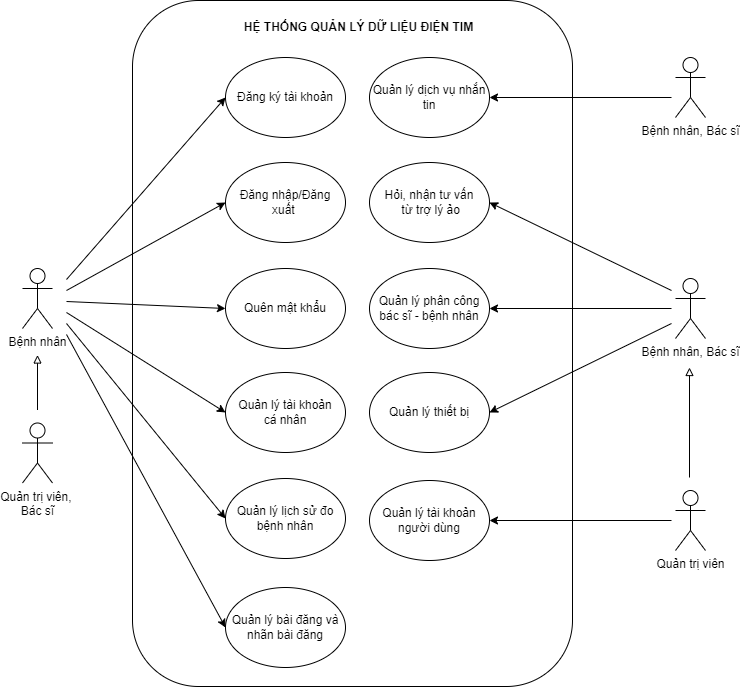
\includegraphics[width=16cm,height=14cm]{Images/use_case/use_case_general.png}
    \caption[Sơ đồ use case tổng quát của hệ thống]{\bfseries \fontsize{12pt}{0pt}
    \selectfont Sơ đồ use case tổng quát của hệ thống}
    \label{use_case_general} %đặt tên cho ảnh
  \end{figure}

\subsubsection{Use case chức năng đăng ký tài khoản}
  \begin{figure}[H]
    \centering
    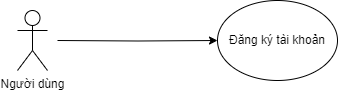
\includegraphics[width=9cm,height=2.5cm]{Images/use_case/use_case_register.png}
    \caption[Sơ đồ use case chức năng đăng ký tài khoản]{\bfseries \fontsize{12pt}{0pt}
    \selectfont Sơ đồ use case chức năng đăng ký tài khoản}
    \label{use_case_register} %đặt tên cho ảnh
  \end{figure}

  \begin{table}[H]
    \caption{\bfseries \fontsize{12pt}{0pt}\selectfont Bảng phân tích use case chức năng đăng ký tài khoản}
    \centering
    \begin{tabularx}{0.9\textwidth}{|c|X|}
      \hline
      \textbf{Tên chức năng} & \textbf{Đăng ký tài khoản} \\
      \hline
      Tác nhân & Bệnh nhân, Bác sĩ, Quản trị viên \\
      \hline
      Mô tả & Cho phép người dùng đăng ký tài khoản để truy cập vào các tài nguyên của hệ thống 
       \\
      \hline
      Điều kiện trước & Người dùng cần có kết nối Internet \\
      \hline
      Dòng sự kiện chính & 
      % \begin{tabular}{@{}l@{}}
        Chi tiết luồng sự kiện được thể hiện ở Hình \ref{activity_register}, Hình \ref{sequence_register} 
        \\
      % \end{tabular} \\
      \hline
    \end{tabularx}
  \end{table}
  Dưới đây là sơ đồ mô tả hoạt động cho chức năng đăng ký tài khoản
  \begin{figure}[H]
    \centering
    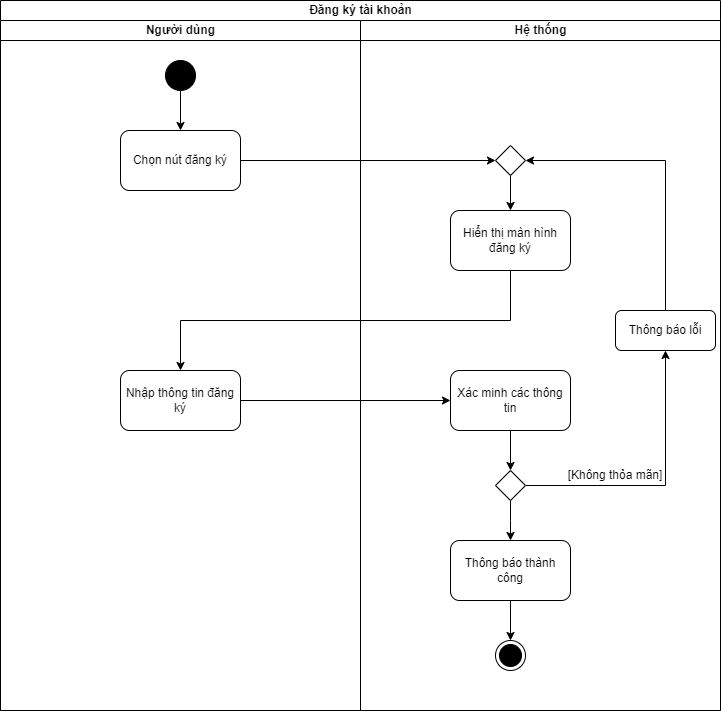
\includegraphics[width=13.5cm,height=13cm]{Images/activity/activity_register.png}
    \caption[Sơ đồ hoạt động chức năng đăng ký tài khoản]{\bfseries \fontsize{12pt}{0pt}
    \selectfont Sơ đồ hoạt động chức năng đăng ký tài khoản}
    \label{activity_register} %đặt tên cho ảnh
  \end{figure}

\subsubsection{Use case chức năng đăng nhập/đăng xuất }
  \begin{figure}[H]
    \centering
    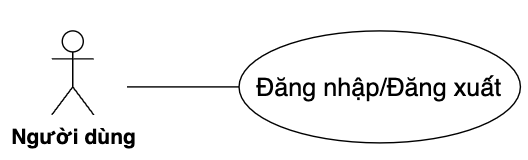
\includegraphics[width=9cm,height=2.5cm]{Images/use_case/use_case_login.png}
    \caption[Sơ đồ use case chức năng đăng nhập/đăng xuất]{\bfseries \fontsize{12pt}{0pt}
    \selectfont Sơ đồ use case chức năng đăng nhập/đăng xuất}
    \label{use_case_login_logout} %đặt tên cho ảnh
  \end{figure}

  \begin{table}[H]
    \caption{\bfseries \fontsize{12pt}{0pt}\selectfont Bảng phân tích use case chức năng đăng nhập/đăng xuất}
    \centering
    \begin{tabularx}{0.9\textwidth}{|c|X|}
      \hline
      \textbf{Tên chức năng} & \textbf{Đăng nhập/Đăng xuất} \\
      \hline
      Tác nhân & Bệnh nhân, Bác sĩ, Quản trị viên \\
      \hline
      Mô tả & Cho phép người dùng sử dụng tài khoản để truy cập vào các tài nguyên của hệ thống và có thể đăng xuất hệ thống
       \\
      \hline
      Điều kiện trước & Người dùng cần có kết nối Internet \\
      \hline
      Dòng sự kiện chính & 
      % \begin{tabular}{@{}l@{}}
        Chi tiết luồng sự kiện được thể hiện ở Hình \ref{activity_login}, Hình \ref{activity_logout},  
        Hình \ref{sequence_login}, Hình \ref{sequence_logout}
        \\
      % \end{tabular} \\
      \hline
    \end{tabularx}
  \end{table}
  Dưới đây là sơ đồ hoạt động dành cho chức năng đăng nhập và đăng xuất
  
  \begin{figure}[H]
    \centering
    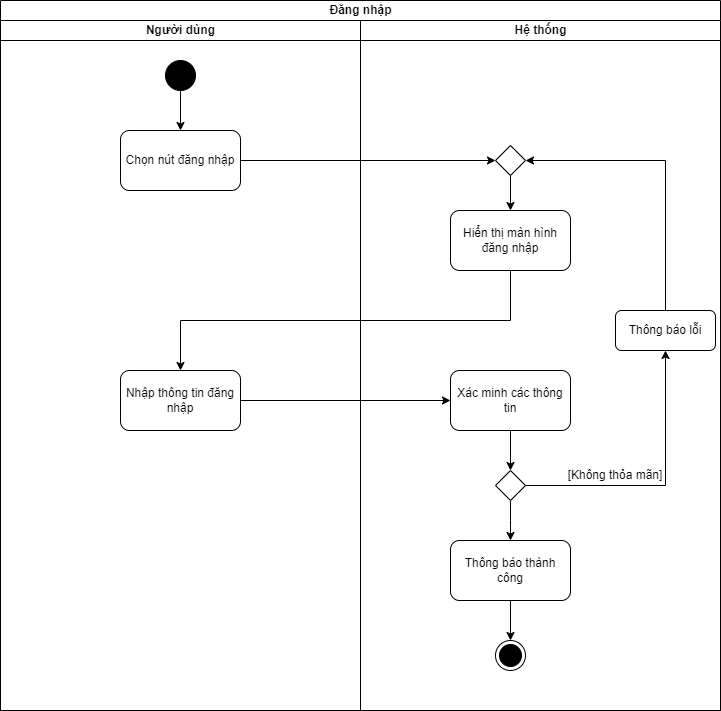
\includegraphics[width=13.5cm,height=13cm]{Images/activity/activity_login.png}
    \caption[Sơ đồ hoạt động chức năng đăng nhập]{\bfseries \fontsize{12pt}{0pt}
    \selectfont Sơ đồ hoạt động chức năng đăng nhập}
    \label{activity_login} %đặt tên cho ảnh
  \end{figure}

  \begin{figure}[H]
    \centering
    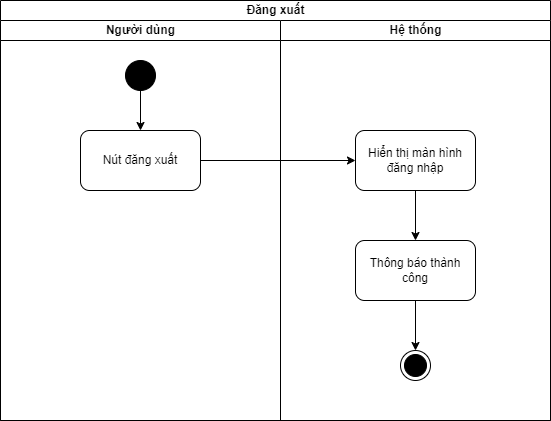
\includegraphics[width=11.5cm,height=9.5cm]{Images/activity/activity_logout.png}
    \caption[Sơ đồ hoạt động chức năng đăng xất]{\bfseries \fontsize{12pt}{0pt}
    \selectfont Sơ đồ hoạt động chức năng đăng xuất}
    \label{activity_logout} %đặt tên cho ảnh
  \end{figure}

\subsubsection{Use case chức năng quên mật khẩu}
  \begin{figure}[H]
    \centering
    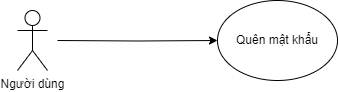
\includegraphics[width=9cm,height=2.5cm]{Images/use_case/use_case_forgot_password.png}
    \caption[Sơ đồ use case chức năng quên mật khẩu]{\bfseries \fontsize{12pt}{0pt}
    \selectfont Sơ đồ use case chức năng quên mật khẩu}
    \label{use_case_forget_password} %đặt tên cho ảnh
  \end{figure}

  \begin{table}[H]
    \caption{\bfseries \fontsize{12pt}{0pt}\selectfont Bảng phân tích use case chức năng quên mật khẩu}
    \centering
    \begin{tabularx}{0.9\textwidth}{|c|X|}
      \hline
      \textbf{Tên chức năng} & \textbf{Quên mật khẩu} \\
      \hline
      Tác nhân & Bệnh nhân, Bác sĩ, Quản trị viên \\
      \hline
      Mô tả & Cho phép người dùng lấy lại mật khẩu tài khoản thông qua email
       \\
      \hline
      Điều kiện trước & Người dùng cần có kết nối Internet và truy cập vào email đăng ký \\
      \hline
      Dòng sự kiện chính & 
      % \begin{tabular}{@{}l@{}}
        Chi tiết luồng sự kiện được thể hiện ở Hình \ref{activity_forgot_password}, Hình \ref{sequence_forgot_pass} 
        \\
      % \end{tabular} \\
      \hline
    \end{tabularx}
  \end{table}
  Dưới đây là sơ đồ hoạt động mô tả chức năng quên mật khẩu
  \begin{figure}[H]
    \centering
    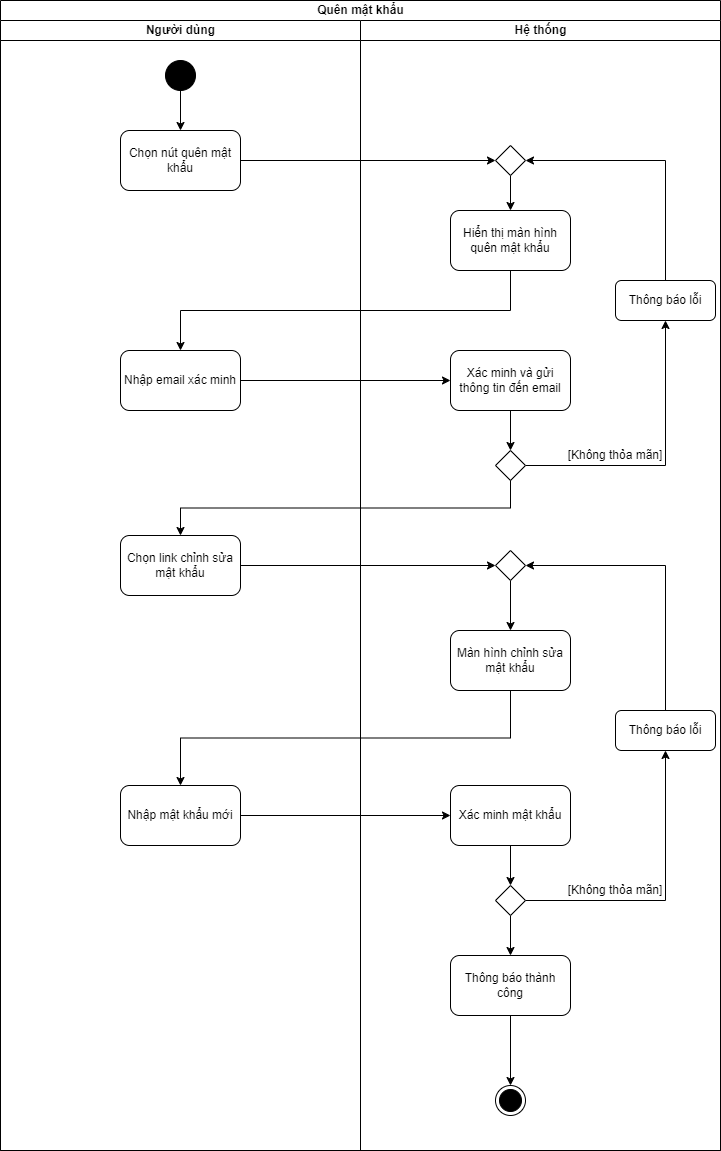
\includegraphics[width=13cm,height=18.5cm]{Images/activity/activity_forgot_pass.png}
    \caption[Sơ đồ hoạt động chức năng quên mật khẩu]{\bfseries \fontsize{12pt}{0pt}
    \selectfont Sơ đồ hoạt động chức năng quên mật khẩu}
    \label{activity_forgot_password} %đặt tên cho ảnh
  \end{figure}

\subsubsection{Use case chức năng quản lý tài khoản cá nhân}
  \begin{figure}[H]
    \centering
    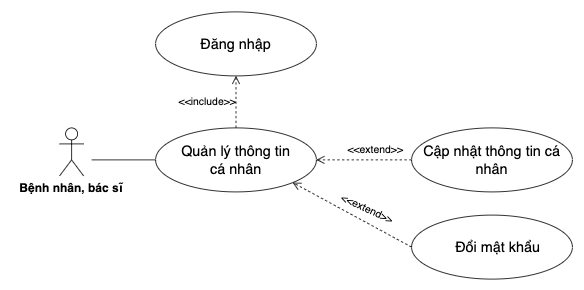
\includegraphics[width=12cm,height=6cm]{Images/use_case/use_case_manage_info.png}
    \caption[Sơ đồ use case chức năng quản lý tài khoản cá nhân]{\bfseries \fontsize{12pt}{0pt}
    \selectfont Sơ đồ use case chức năng quản lý tài khoản cá nhân}
    \label{use_case_manage_info} %đặt tên cho ảnh
  \end{figure}

  \begin{table}[H]
    \caption{\bfseries \fontsize{12pt}{0pt}\selectfont Bảng phân tích use case chức năng quản lý tài khoản cá nhân}
    \centering
    \begin{tabularx}{0.9\textwidth}{|c|X|}
      \hline
      \textbf{Tên chức năng} & \textbf{Quản lý tài khoản cá nhân} \\
      \hline
      Tác nhân & Bệnh nhân, Bác sĩ, Quản trị viên \\
      \hline
      Mô tả & Cho phép người dùng xem, thay đổi thông tin cá nhân như số điện thoại, email, tên hiển thị
       \\
      \hline
      Điều kiện trước & Người dùng cần có kết nối Internet và đăng nhập \\
      \hline
      Dòng sự kiện chính & 
      % \begin{tabular}{@{}l@{}}
        Chi tiết luồng sự kiện được thể hiện ở Hình \ref{activity_manage_info}, Hình \ref{sequence_account} 
        \\
      % \end{tabular} \\
      \hline
    \end{tabularx}
  \end{table}
  Dưới đây là sơ đồ hoạt động mô tả chức năng quản lý tài khoản cá nhân
  \begin{figure}[H]
    \centering
    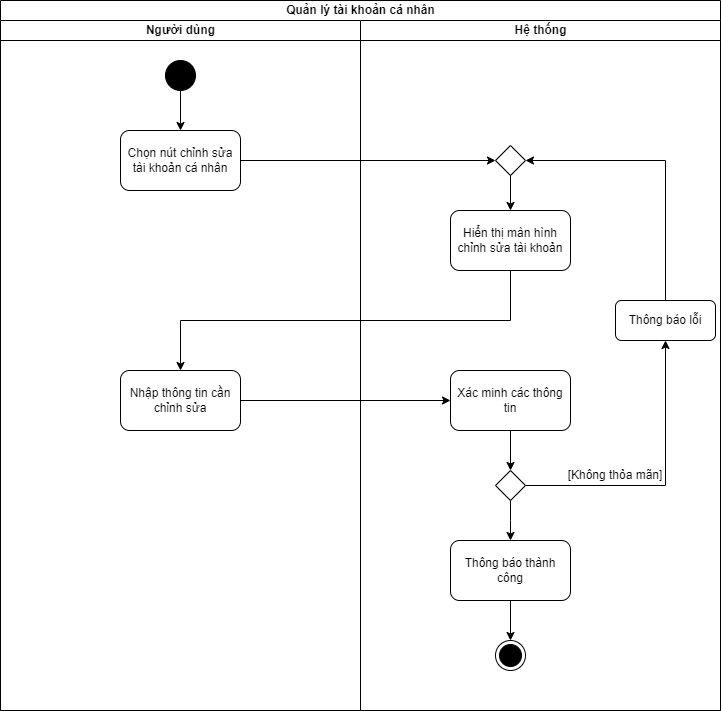
\includegraphics[width=13.5cm,height=14cm]{Images/activity/activity_manage_info.png}
    \caption[Sơ đồ hoạt động chức năng quản lý tài khoản cá nhân]{\bfseries \fontsize{12pt}{0pt}
    \selectfont Sơ đồ hoạt động chức năng quản lý tài khoản cá nhân}
    \label{activity_manage_info} %đặt tên cho ảnh
  \end{figure}

\subsubsection{Use case chức năng xem lịch sử các lần đo}
  \begin{figure}[H]
    \centering
    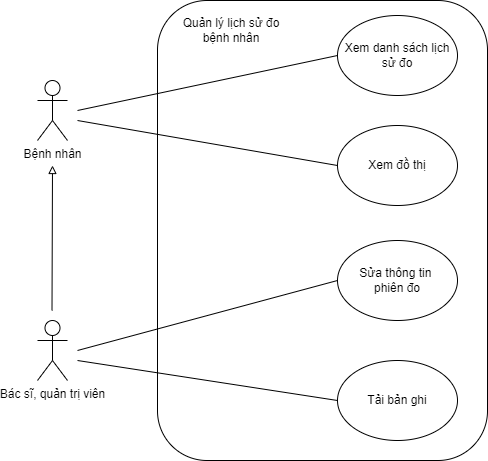
\includegraphics[width=12cm,height=11cm]{Images/use_case/use_case_view_history_record.png}
    \caption[Sơ đồ use case chức năng xem lịch sử các lần đo]{\bfseries \fontsize{12pt}{0pt}
    \selectfont Sơ đồ use case chức năng xem lịch sử các lần đo}
    \label{use_case_view_history_record} %đặt tên cho ảnh
  \end{figure}

  \begin{table}[H]
    \caption{\bfseries \fontsize{12pt}{0pt}\selectfont Bảng phân tích use case chức năng xem danh sách lịch sử đo}
    \centering
    \begin{tabularx}{0.9\textwidth}{|c|X|}
      \hline
      \textbf{Tên chức năng} & \textbf{Xem danh sách lịch sử đo} \\
      \hline
      Tác nhân & Bệnh nhân, Bác sĩ, Quản trị viên \\
      \hline
      Mô tả & Cho phép bệnh nhân xem lịch sử các lần đo điện tim, bác sĩ xem được lịch sử các lần đo của bệnh nhân
      mà mình quản lý.\\
      \hline
      Điều kiện trước & Người dùng cần có kết nối Internet và đã đăng nhập \\
      \hline
      Dòng sự kiện chính & 
      % \begin{tabular}{@{}l@{}}
        Chi tiết luồng sự kiện được thể hiện ở Hình \ref{activity_record_history}, Hình \ref{sequence_manage_record}
        \\
      % \end{tabular} \\
      \hline
    \end{tabularx}
  \end{table}

  \begin{table}[H]
    \caption{\bfseries \fontsize{12pt}{0pt}\selectfont Bảng phân tích use case chức năng xem đồ thị}
    \centering
    \begin{tabularx}{0.9\textwidth}{|c|X|}
      \hline
      \textbf{Tên chức năng} & \textbf{Xem đồ thị} \\
      \hline
      Tác nhân & Bệnh nhân, Bác sĩ, Quản trị viên \\
      \hline
      Mô tả & Cho phép bệnh nhân xem đồ thị trong lần đo điện tim, bác sĩ xem được đồ thị của bệnh nhân
      mà mình quản lý.\\
      \hline
      Điều kiện trước & Người dùng cần có kết nối Internet và đã đăng nhập \\
      \hline
      Dòng sự kiện chính & 
      % \begin{tabular}{@{}l@{}}
        Chi tiết luồng sự kiện được thể hiện ở Hình \ref{activity_record_history}, Hình \ref{sequence_manage_record}, Hình \ref{getEcgRecordsByDoctor} 
        \\
      % \end{tabular} \\
      \hline
    \end{tabularx}
  \end{table}

  \begin{table}[H]
    \caption{\bfseries \fontsize{12pt}{0pt}\selectfont Bảng phân tích use case chức năng tải bản ghi dữ liệu đo}
    \centering
    \begin{tabularx}{0.9\textwidth}{|c|X|}
      \hline
      \textbf{Tên chức năng} & \textbf{Tải bản ghi dữ liệu đo} \\
      \hline
      Tác nhân & Bác sĩ, Quản trị viên \\
      \hline
      Mô tả & Cho phép bác sĩ tải bản ghi dữ liệu đo của bệnh nhân
      mà mình quản lý, quản trị viên có thể tải bản đo dữ liệu bất kì.\\
      \hline
      Điều kiện trước & Người dùng cần có kết nối Internet và đã đăng nhập \\
      \hline
      Dòng sự kiện chính & 
      % \begin{tabular}{@{}l@{}}
        Chi tiết luồng sự kiện được thể hiện ở Hình \ref{activity_record_history}, Hình \ref{sequence_manage_record}, Hình \ref{getEcgRecordsByDoctor} 
        \\
      % \end{tabular} \\
      \hline
    \end{tabularx}
  \end{table}

  Dưới đây là sơ đồ hoạt động mô tả chức năng xem lịch sử các lần đo
  \begin{figure}[H]
    \centering
    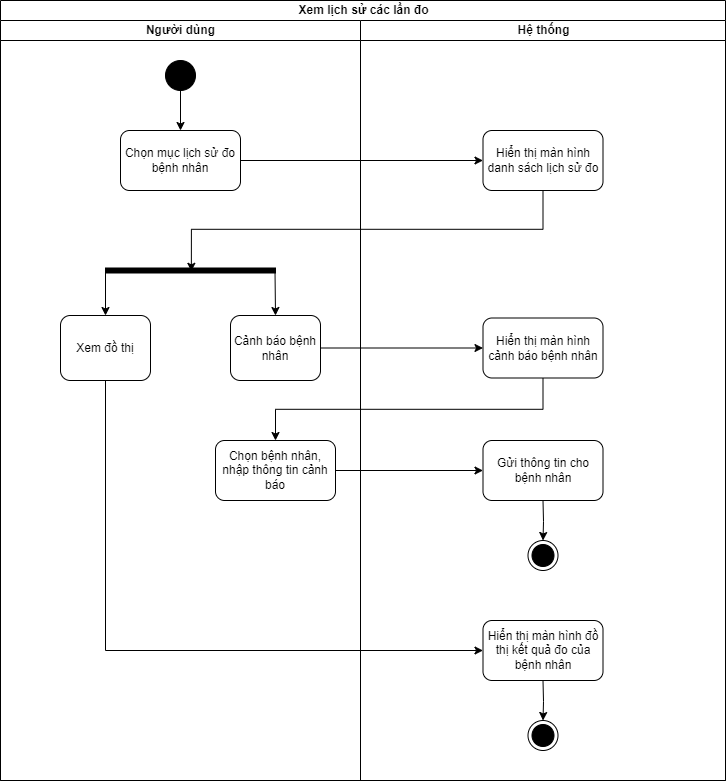
\includegraphics[width=13.5cm,height=15cm]{Images/activity/activity_record_history.png}
    \caption[Sơ đồ hoạt động chức năng xem lịch sử các lần đo]{\bfseries \fontsize{12pt}{0pt}
    \selectfont Sơ đồ hoạt động chức năng xem lịch sử các lần đo}
    \label{activity_record_history} %đặt tên cho ảnh
  \end{figure}

\subsubsection{Use case chức năng quản lí dịch vụ nhắn tin}
  \begin{figure}[H]
    \centering
    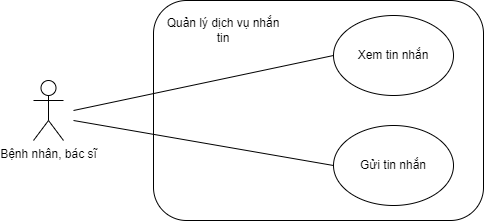
\includegraphics[width=12cm,height=8cm]{Images/use_case/use_case_send_receive_message.png}
    \caption[Sơ đồ use case chức năng quản lí dịch vụ nhắn tin]{\bfseries \fontsize{12pt}{0pt}
    \selectfont Sơ đồ use case chức năng quản lí dịch vụ nhắn tin}
    \label{use_case_chat} %đặt tên cho ảnh
  \end{figure}

  \begin{table}[H]
    \caption{\bfseries \fontsize{12pt}{0pt}\selectfont Bảng phân tích use case chức năng quản lí dịch vụ nhắn tin}
    \centering
    \begin{tabularx}{0.9\textwidth}{|c|X|}
      \hline
      \textbf{Tên chức năng} & \textbf{Xem/Gửi tin nhắn} \\
      \hline
      Tác nhân & Bệnh nhân, Bác sĩ \\
      \hline
      Mô tả & Cho phép bệnh nhân chat với bác sĩ phụ trách và bác sĩ có thể chat với bệnh nhân mà mình phụ trách \\
      \hline
      Điều kiện trước & Người dùng cần có kết nối Internet và đã đăng nhập \\
      \hline
      Dòng sự kiện chính & 
      % \begin{tabular}{@{}l@{}}
        Chi tiết luồng sự kiện được thể hiện ở Hình \ref{activity_chat}, Hình \ref{sequence_chat} 
        \\
      % \end{tabular} \\
      \hline
    \end{tabularx}
  \end{table}
  Dưới đây là sơ đồ hoạt động mô tả chức năng quản lý dịch vụ nhắn tin
  \begin{figure}[H]
    \centering
    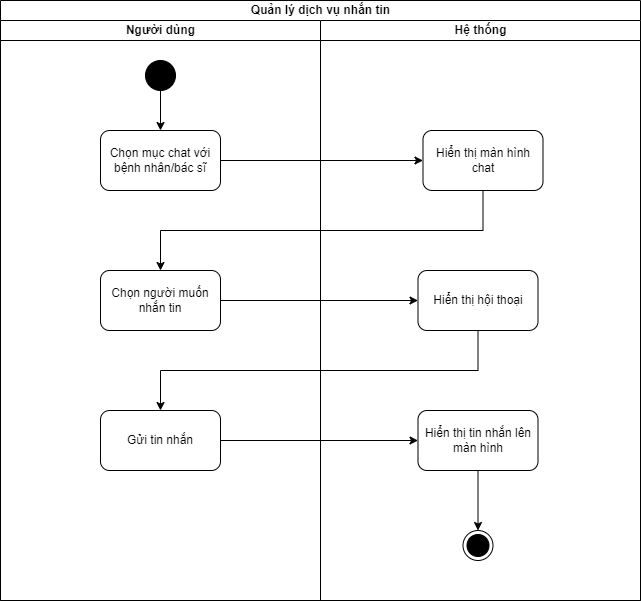
\includegraphics[width=11.5cm,height=11cm]{Images/activity/activity_chat.png}
    \caption[Sơ đồ hoạt động chức năng quản lý dịch vụ nhắn tin]{\bfseries \fontsize{12pt}{0pt}
    \selectfont Sơ đồ hoạt động chức năng quản lý dịch vụ nhắn tin}
    \label{activity_chat} %đặt tên cho ảnh
  \end{figure}

  \begin{table}[H]
    \caption{\bfseries \fontsize{12pt}{0pt}\selectfont Bảng phân tích use case chức năng gửi tin nhắn cho trợ lý ảo}
    \centering
    \begin{tabularx}{0.9\textwidth}{|c|X|}
      \hline
      \textbf{Tên chức năng} & \textbf{Gửi tin nhắn cho trợ lý ảo} \\
      \hline
      Tác nhân & Bệnh nhân \\
      \hline
      Mô tả & Cho phép bệnh nhân chat với chat bot trợ lý ảo \\
      \hline
      Điều kiện trước & Người dùng cần có kết nối Internet và đã đăng nhập \\
      \hline
      Dòng sự kiện chính & 
      % \begin{tabular}{@{}l@{}}
        Chi tiết luồng sự kiện được thể hiện ở Hình \ref{activity_chat_ai}, Hình \ref{sequence_chat_ai} 
        \\
      % \end{tabular} \\
      \hline
    \end{tabularx}
  \end{table}  
  Dưới đây là sơ đồ hoạt động mô tả chức năng tư vấn từ trợ lý ảo
  \begin{figure}[H]
    \centering
    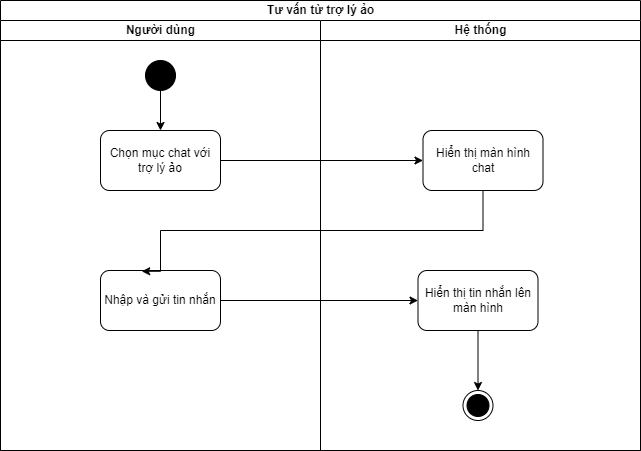
\includegraphics[width=11.5cm,height=8.5cm]{Images/activity/activity_chat_ai.png}
    \caption[Sơ đồ hoạt động chức năng tư vấn từ trợ lý ảo]{\bfseries \fontsize{12pt}{0pt}
    \selectfont Sơ đồ hoạt động chức năng tư vấn từ trợ lý ảo}
    \label{activity_chat_ai} %đặt tên cho ảnh
  \end{figure}

\subsubsection{Use case chức năng quản lý bệnh nhân}
  \begin{figure}[H]
    \centering
    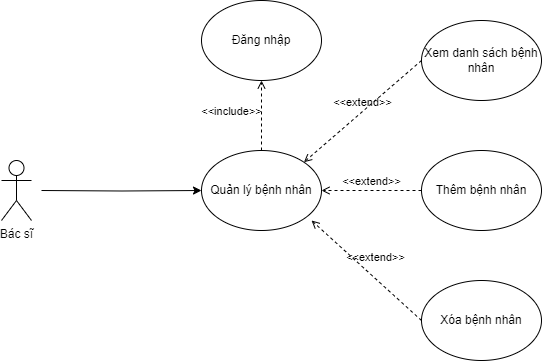
\includegraphics[width=12cm,height=8.5cm]{Images/use_case/use_case_manage_patients.png}
    \caption[Sơ đồ use case chức năng quản lý bệnh nhân]{\bfseries \fontsize{12pt}{0pt}
    \selectfont Sơ đồ use case chức năng quản lý bệnh nhân}
    \label{use_case_patient_management} %đặt tên cho ảnh
  \end{figure}

  \begin{table}[H]
    \caption{\bfseries \fontsize{12pt}{0pt}\selectfont Bảng phân tích use case chức năng xem danh sách bệnh nhân}
    \centering
    \begin{tabularx}{0.9\textwidth}{|c|X|}
      \hline
      \textbf{Tên chức năng} & \textbf{Xem danh sách bệnh nhân} \\
      \hline
      Tác nhân & Bác sĩ \\
      \hline
      Mô tả & Cho phép bác sĩ thực hiện hành động xem danh sách bệnh nhân của mình \\
      \hline
      Điều kiện trước & Người dùng cần có kết nối Internet và đã đăng nhập \\
      \hline
      Dòng sự kiện chính & 
      % \begin{tabular}{@{}l@{}}
        Chi tiết luồng sự kiện được thể hiện ở Hình \ref{activity_patient_management}, Hình \ref{sequence_manage_patient}
        \\
      % \end{tabular} \\
      \hline
    \end{tabularx}
  \end{table}

  \begin{table}[H]
    \caption{\bfseries \fontsize{12pt}{0pt}\selectfont Bảng phân tích use case chức năng sửa thông tin bệnh nhân}
    \centering
    \begin{tabularx}{0.9\textwidth}{|c|X|}
      \hline
      \textbf{Tên chức năng} & \textbf{Sửa thông tin bệnh nhân} \\
      \hline
      Tác nhân & Bác sĩ \\
      \hline
      Mô tả & Cho phép bác sĩ thực hiện hành động sửa thông tin bệnh nhân trong danh sách bệnh nhân của mình \\
      \hline
      Điều kiện trước & Người dùng cần có kết nối Internet và đã đăng nhập \\
      \hline
      Dòng sự kiện chính & 
      % \begin{tabular}{@{}l@{}}
        Chi tiết luồng sự kiện được thể hiện ở Hình \ref{activity_patient_management}, Hình \ref{sequence_manage_edit_patient}
        \\
      % \end{tabular} \\
      \hline
    \end{tabularx}
  \end{table}

  \begin{table}[H]
    \caption{\bfseries \fontsize{12pt}{0pt}\selectfont Bảng phân tích use case chức năng xóa bệnh nhân}
    \centering
    \begin{tabularx}{0.9\textwidth}{|c|X|}
      \hline
      \textbf{Tên chức năng} & \textbf{Xóa bệnh nhân} \\
      \hline
      Tác nhân & Bác sĩ \\
      \hline
      Mô tả & Cho phép bác sĩ thực hiện hành động xóa bệnh nhân trong danh sách bệnh nhân của mình \\
      \hline
      Điều kiện trước & Người dùng cần có kết nối Internet và đã đăng nhập \\
      \hline
      Dòng sự kiện chính & 
      % \begin{tabular}{@{}l@{}}
        Chi tiết luồng sự kiện được thể hiện ở Hình \ref{activity_patient_management}, Hình \ref{sequence_manage_delete_patient}
        \\
      % \end{tabular} \\
      \hline
    \end{tabularx}
  \end{table}

  Dưới đây là sơ đồ hoạt động mô tả chức năng quản lý bệnh nhân
  \begin{figure}[H]
    \centering
    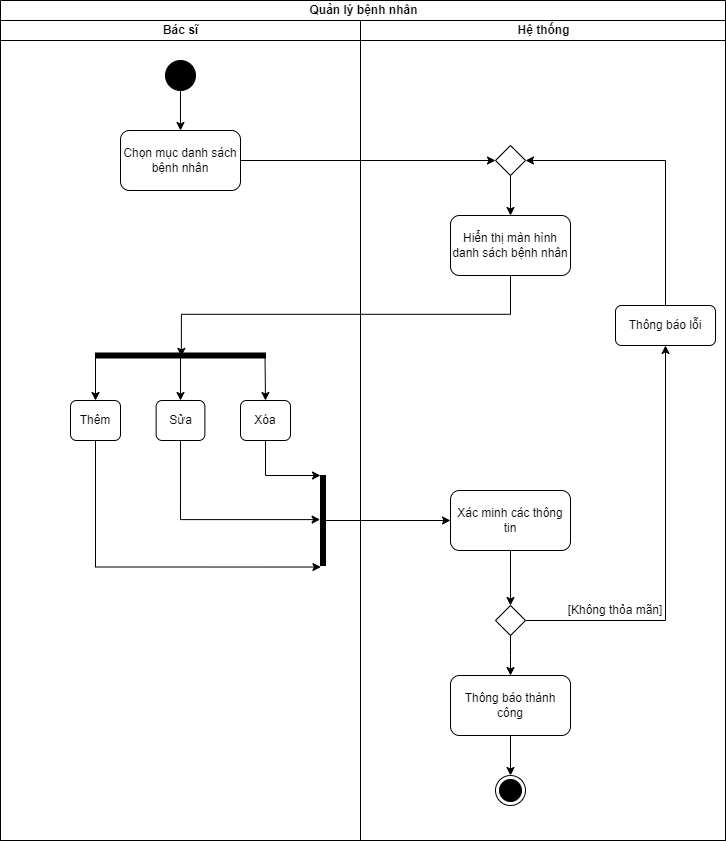
\includegraphics[width=13.5cm,height=16cm]{Images/activity/activity_manage_patient.png}
    \caption[Sơ đồ hoạt động chức năng quản lý bệnh nhân]{\bfseries \fontsize{12pt}{0pt}
    \selectfont Sơ đồ hoạt động chức năng quản lý bệnh nhân}
    \label{activity_patient_management} %đặt tên cho ảnh
  \end{figure}

\subsubsection{Use case chức năng quản lý thiết bị}
  \begin{figure}[H]
    \centering
    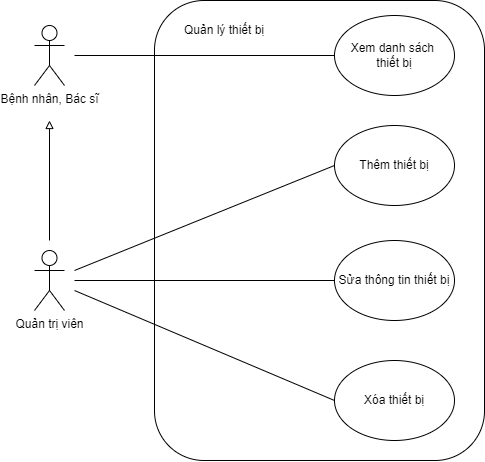
\includegraphics[width=12cm,height=11cm]{Images/use_case/use_case_manage_device.png}
    \caption[Sơ đồ use case chức năng quản lý thiết bị]{\bfseries \fontsize{12pt}{0pt}
    \selectfont Sơ đồ use case chức năng quản lý thiết bị}
    \label{use_case_device_management} %đặt tên cho ảnh
  \end{figure}

  \begin{table}[H]
    \caption{\bfseries \fontsize{12pt}{0pt}\selectfont Bảng phân tích use case chức năng xem danh sách thiết bị}
    \centering
    \begin{tabularx}{0.9\textwidth}{|c|X|}
      \hline
      \textbf{Tên chức năng} & \textbf{Xem danh sách thiết bị} \\
      \hline
      Tác nhân & Quản trị viên \\
      \hline
      Mô tả & Cho phép quản trị thực hiện hành động xem thông tin danh sách thiết bị \\
      \hline
      Điều kiện trước & Người dùng cần có kết nối Internet và đã đăng nhập \\
      \hline
      Dòng sự kiện chính & 
      % \begin{tabular}{@{}l@{}}
        Chi tiết luồng sự kiện được thể hiện ở Hình \ref{activity_device_management}, Hình \ref{sequence_manage_device} 
        \\
      % \end{tabular} \\
      \hline
    \end{tabularx}
  \end{table}

  \begin{table}[H]
    \caption{\bfseries \fontsize{12pt}{0pt}\selectfont Bảng phân tích use case chức năng thêm thiết bị}
    \centering
    \begin{tabularx}{0.9\textwidth}{|c|X|}
      \hline
      \textbf{Tên chức năng} & \textbf{Thêm thiết bị} \\
      \hline
      Tác nhân & Quản trị viên \\
      \hline
      Mô tả & Cho phép quản trị thực hiện hành động thêm thiết bị vào danh sách thiết bị\\
      \hline
      Điều kiện trước & Người dùng cần có kết nối Internet và đã đăng nhập \\
      \hline
      Dòng sự kiện chính & 
      % \begin{tabular}{@{}l@{}}
        Chi tiết luồng sự kiện được thể hiện ở Hình \ref{activity_device_management}, Hình \ref{sequence_manage_add_device}
        \\
      % \end{tabular} \\
      \hline
    \end{tabularx}
  \end{table}

  \begin{table}[H]
    \caption{\bfseries \fontsize{12pt}{0pt}\selectfont Bảng phân tích use case chức năng sửa thông tin thiết bị}
    \centering
    \begin{tabularx}{0.9\textwidth}{|c|X|}
      \hline
      \textbf{Tên chức năng} & \textbf{Sửa thông tin thiết bị} \\
      \hline
      Tác nhân & Quản trị viên \\
      \hline
      Mô tả & Cho phép quản trị thực hiện hành động sửa thông tin thiết bị \\
      \hline
      Điều kiện trước & Người dùng cần có kết nối Internet và đã đăng nhập \\
      \hline
      Dòng sự kiện chính & 
      % \begin{tabular}{@{}l@{}}
        Chi tiết luồng sự kiện được thể hiện ở Hình \ref{activity_device_management}, Hình \ref{sequence_manage_edit_device}
        \\
      % \end{tabular} \\
      \hline
    \end{tabularx}
  \end{table}

  \begin{table}[H]
    \caption{\bfseries \fontsize{12pt}{0pt}\selectfont Bảng phân tích use case chức năng xóa thiết bị}
    \centering
    \begin{tabularx}{0.9\textwidth}{|c|X|}
      \hline
      \textbf{Tên chức năng} & \textbf{Xóa thiết bị} \\
      \hline
      Tác nhân & Quản trị viên \\
      \hline
      Mô tả & Cho phép quản trị thực hiện hành động xóa thiết bị \\
      \hline
      Điều kiện trước & Người dùng cần có kết nối Internet và đã đăng nhập \\
      \hline
      Dòng sự kiện chính & 
      % \begin{tabular}{@{}l@{}}
        Chi tiết luồng sự kiện được thể hiện ở Hình \ref{activity_device_management}, Hình \ref{sequence_manage_delete_device}
        \\
      % \end{tabular} \\
      \hline
    \end{tabularx}
  \end{table}

  Dưới đây là sơ đồ hoạt động mô tả chức năng quản lý thiết bị
  \begin{figure}[H]
    \centering
    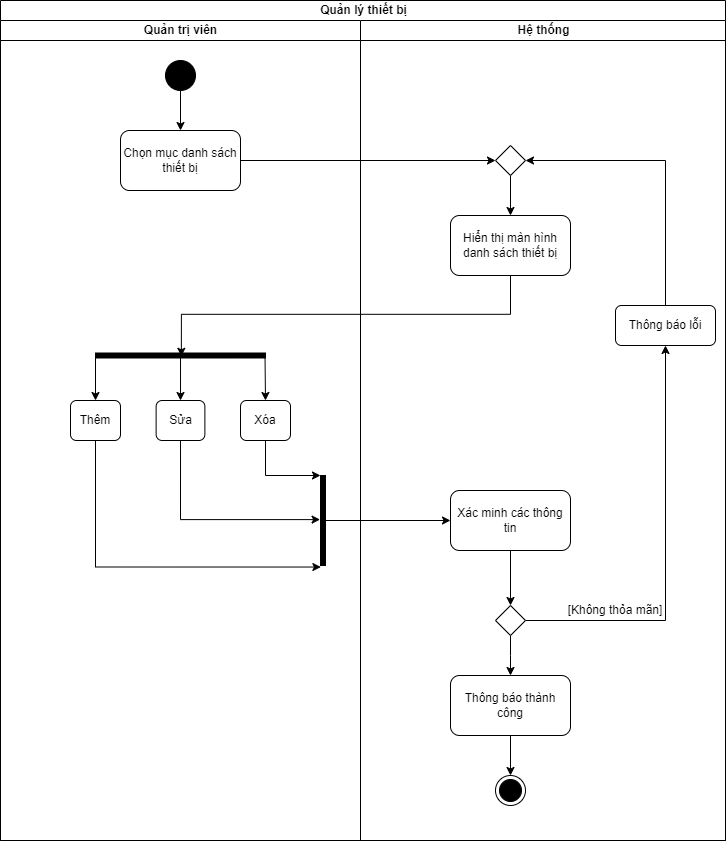
\includegraphics[width=13.5cm,height=16cm]{Images/activity/activity_manage_device.png}
    \caption[Sơ đồ hoạt động chức năng quản lý thiết bị]{\bfseries \fontsize{12pt}{0pt}
    \selectfont Sơ đồ hoạt động chức năng quản lý thiết bị}
    \label{activity_device_management} %đặt tên cho ảnh
  \end{figure}


\subsubsection{Use case chức năng quản lý tài khoản người dùng}
  \begin{figure}[H]
    \centering
    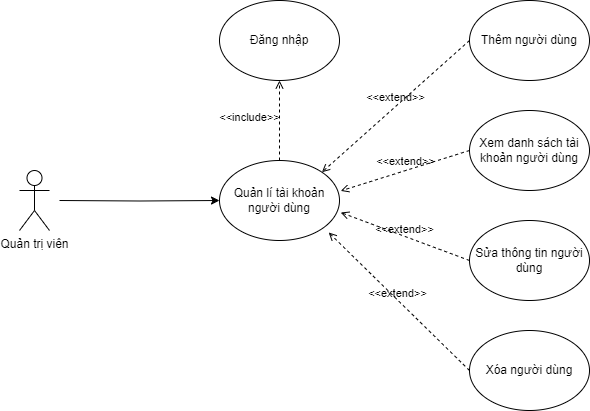
\includegraphics[width=12cm,height=12.5cm]{Images/use_case/use_case_manage_users.png}
    \caption[Sơ đồ use case chức năng tài khoản người dùng]{\bfseries \fontsize{12pt}{0pt}
    \selectfont Sơ đồ use case chức năng tài khoản người dùng}
    \label{use_case_user_management} %đặt tên cho ảnh
  \end{figure}

  \begin{table}[H]
    \caption{\bfseries \fontsize{12pt}{0pt}\selectfont Bảng phân tích use case chức năng xem danh sách tài khoản người dùng}
    \centering
    \begin{tabularx}{0.9\textwidth}{|c|X|}
      \hline
      \textbf{Tên chức năng} & \textbf{Xem danh sách tài khoản người dùng} \\
      \hline
      Tác nhân & Quản trị viên \\
      \hline
      Mô tả & Cho phép quản trị thực hiện hành động xem danh sách tài khoản người dùng \\
      \hline
      Điều kiện trước & Người dùng cần có kết nối Internet và đã đăng nhập \\
      \hline
      Dòng sự kiện chính & 
      % \begin{tabular}{@{}l@{}}
        Chi tiết luồng sự kiện được thể hiện ở Hình \ref{activity_user_management}, Hình \ref{sequence_manage_user}
        \\
      % \end{tabular} \\
      \hline
    \end{tabularx}
  \end{table}

  \begin{table}[H]
    \caption{\bfseries \fontsize{12pt}{0pt}\selectfont Bảng phân tích use case chức năng thêm người dùng}
    \centering
    \begin{tabularx}{0.9\textwidth}{|c|X|}
      \hline
      \textbf{Tên chức năng} & \textbf{Thêm người dùng} \\
      \hline
      Tác nhân & Quản trị viên \\
      \hline
      Mô tả & Cho phép quản trị thực hiện hành động thêm người dùng \\
      \hline
      Điều kiện trước & Người dùng cần có kết nối Internet và đã đăng nhập \\
      \hline
      Dòng sự kiện chính & 
      % \begin{tabular}{@{}l@{}}
        Chi tiết luồng sự kiện được thể hiện ở Hình \ref{activity_user_management}, Hình \ref{sequence_manage_add_user}
        \\
      % \end{tabular} \\
      \hline
    \end{tabularx}
  \end{table}

  \begin{table}[H]
    \caption{\bfseries \fontsize{12pt}{0pt}\selectfont Bảng phân tích use case chức năng sửa thông tin người dùng}
    \centering
    \begin{tabularx}{0.9\textwidth}{|c|X|}
      \hline
      \textbf{Tên chức năng} & \textbf{Sửa thông tin người dùng} \\
      \hline
      Tác nhân & Quản trị viên \\
      \hline
      Mô tả & Cho phép quản trị thực hiện hành động sửa thông tin người dùng \\
      \hline
      Điều kiện trước & Người dùng cần có kết nối Internet và đã đăng nhập \\
      \hline
      Dòng sự kiện chính & 
      % \begin{tabular}{@{}l@{}}
        Chi tiết luồng sự kiện được thể hiện ở Hình \ref{activity_user_management}, Hình \ref{sequence_manage_edit_user}
        \\
      % \end{tabular} \\
      \hline
    \end{tabularx}
  \end{table}

  \begin{table}[H]
    \caption{\bfseries \fontsize{12pt}{0pt}\selectfont Bảng phân tích use case chức năng xóa người dùng}
    \centering
    \begin{tabularx}{0.9\textwidth}{|c|X|}
      \hline
      \textbf{Tên chức năng} & \textbf{Xóa người dùng} \\
      \hline
      Tác nhân & Quản trị viên \\
      \hline
      Mô tả & Cho phép quản trị thực hiện hành động xóa người dùng \\
      \hline
      Điều kiện trước & Người dùng cần có kết nối Internet và đã đăng nhập \\
      \hline
      Dòng sự kiện chính & 
      % \begin{tabular}{@{}l@{}}
        Chi tiết luồng sự kiện được thể hiện ở Hình \ref{activity_user_management}, Hình \ref{sequence_manage_delete_user} 
        \\
      % \end{tabular} \\
      \hline
    \end{tabularx}
  \end{table}

  \begin{table}[H]
    \caption{\bfseries \fontsize{12pt}{0pt}\selectfont Bảng phân tích use case chức năng quản lý đăng ký tài khoản người dùng}
    \centering
    \begin{tabularx}{0.9\textwidth}{|c|X|}
      \hline
      \textbf{Tên chức năng} & \textbf{Quản lý đăng ký tài khoản người dùng} \\
      \hline
      Tác nhân & Quản trị viên \\
      \hline
      Mô tả & Cho phép quản trị thực hiện hành động quản lý đăng ký đối với tài khoản người dùng \\
      \hline
      Điều kiện trước & Người dùng cần có kết nối Internet và đã đăng nhập \\
      \hline
      Dòng sự kiện chính & 
      % \begin{tabular}{@{}l@{}}
        Chi tiết luồng sự kiện được thể hiện ở Hình \ref{activity_register_management}
        \\
      % \end{tabular} \\
      \hline
    \end{tabularx}
  \end{table}
  Dưới đây là sơ đồ hoạt động mô tả chức năng quản lý tài khoản người dùng
  \begin{figure}[H]
    \centering
    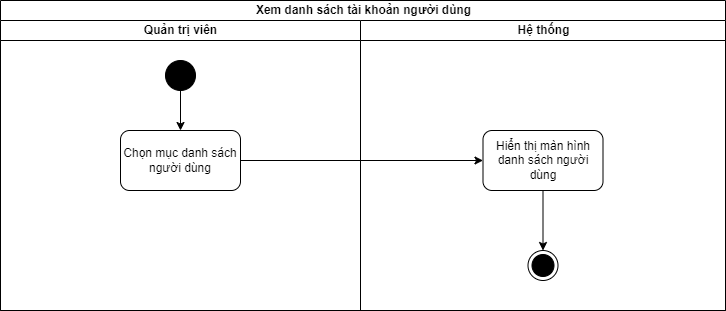
\includegraphics[width=13.5cm,height=16cm]{Images/activity/activity_manage_user.png}
    \caption[Sơ đồ hoạt động chức năng quản lý tài khoản người dùng]{\bfseries \fontsize{12pt}{0pt}
    \selectfont Sơ đồ hoạt động chức năng quản lý tài khoản người dùng}
    \label{activity_user_management} %đặt tên cho ảnh
  \end{figure}

  \begin{figure}[H]
    \centering
    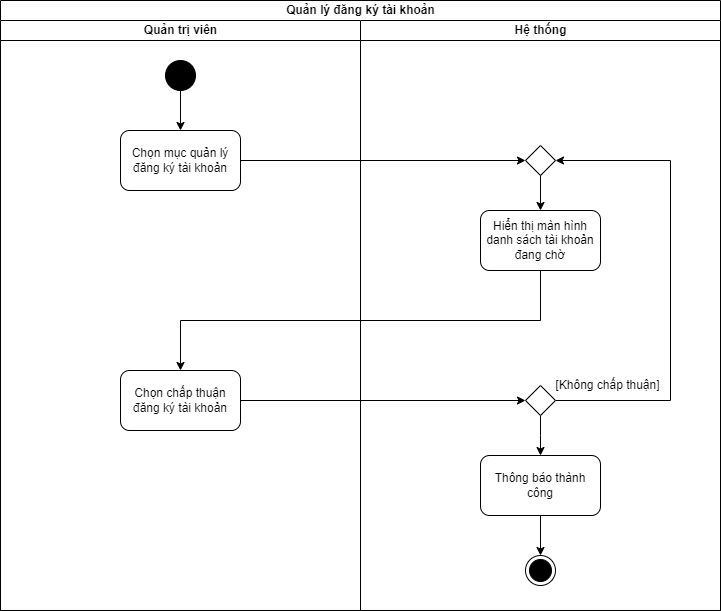
\includegraphics[width=13.5cm,height=11cm]{Images/activity/activity_manage_register.png}
    \caption[Sơ đồ hoạt động chức năng quản lý đăng ký tài khoản người dùng]{\bfseries \fontsize{12pt}{0pt}
    \selectfont Sơ đồ hoạt động chức năng quản lý đăng ký tài khoản người dùng}
    \label{activity_register_management} %đặt tên cho ảnh
  \end{figure}

% \newpage
\subsection{Thẻ CRC (Class - Responsibility - Collaboration Card)}

\subsubsection{Thẻ CRC lớp Người dùng}
  \begin{table}[H]
    \caption{\bfseries \fontsize{12pt}{0pt}\selectfont Thẻ CRC lớp Người dùng}
    \centering
    \begin{tabularx}{0.9\textwidth}{X}
      Mặt trước thẻ
    \end{tabularx}
    \begin{tabularx}{0.9\textwidth}{|X|X|X|}
      \hline
      \textbf{Class name:} Người dùng & \textbf{ID:} 1 & \textbf{Type:} Concrete, Domain \\
      \hline
    \end{tabularx}
    \begin{tabularx}{0.9\textwidth}{|X|X|}
      \textbf{Description:} Đối tượng mô tả thông tin người dùng & \textbf{Associated use case:} 3 \\
      \hline
      \textbf{Responsibility:} & \textbf{Collaboration:} \\
      Thông tin người dùng 
      & 
      Thiết bị
      
      Bản ghi

      Tài khoản
      \\
      \hline
    \end{tabularx}
    \begin{tabularx}{0.9\textwidth}{X}
      Mặt sau thẻ
    \end{tabularx}
    \begin{tabularx}{0.9\textwidth}{|X|X|}
      \hline
      \textbf{Attributes} & \\
      id(String) 
      
      account\_id(String)

      username(String)

      birth(BigInt)

      phone\_number(String)
      & 
      image(String) 
      
      role(Int) 
      
      created\_at(BigInt)

      updated\_at(BigInt)
      \\
      \hline
    \end{tabularx}
    \begin{tabularx}{0.9\textwidth}{|X|}
      \textbf{Relationships} \\
      Generalize:  

      Aggregation: Thiết bị, Bản ghi
      
      Association: Tài khoản 
      \\
      \hline
    \end{tabularx}
  \end{table}

  \subsubsection{Thẻ CRC lớp Thiết bị}
  \begin{table}[H]
    \caption{\bfseries \fontsize{12pt}{0pt}\selectfont Thẻ CRC lớp Thiết bị}
    \centering
    \begin{tabularx}{0.9\textwidth}{X}
      Mặt trước thẻ
    \end{tabularx}
    \begin{tabularx}{0.9\textwidth}{|X|X|X|}
      \hline
      \textbf{Class name:} Thiết bị & \textbf{ID:} 2 & \textbf{Type:} Concrete, Domain \\
      \hline
    \end{tabularx}
    \begin{tabularx}{0.9\textwidth}{|X|X|}
      \textbf{Description:} Đối tượng mô tả thông tin thiết bị & \textbf{Associated use case:} 2 \\
      \hline
      \textbf{Responsibility:} & \textbf{Collaboration:} \\
      Thông tin thiết bị 
      & 
      Người dùng 

      Bản ghi
      \\
      \hline
    \end{tabularx}
    \begin{tabularx}{0.9\textwidth}{X}
      Mặt sau thẻ
    \end{tabularx}
    \begin{tabularx}{0.9\textwidth}{|X|X|}
      \hline
      \textbf{Attributes} & \\
      id(String) 
      
      user\_id(String)

      device\_name(String)

      infomation(String)

      device\_type(Integer)
      & 
      start\_date(BigInt) 
      
      end\_date(BigInt) 
      
      created\_at(BigInt)

      updated\_at(BigInt)
      \\
      \hline
    \end{tabularx}
    \begin{tabularx}{0.9\textwidth}{|X|}
      \textbf{Relationships} \\
      Generalize:  

      Aggregation: Người dùng
      
      Association: Bản ghi
      \\
      \hline
    \end{tabularx}
  \end{table}

\subsubsection{Thẻ CRC lớp Bản ghi}
  \begin{table}[H]
    \caption{\bfseries \fontsize{12pt}{0pt}\selectfont Thẻ CRC lớp Bản ghi}
    \centering
    \begin{tabularx}{0.9\textwidth}{X}
      Mặt trước thẻ
    \end{tabularx}
    \begin{tabularx}{0.9\textwidth}{|X|X|X|}
      \hline
      \textbf{Class name:} Bản ghi & \textbf{ID:} 3 & \textbf{Type:} Concrete, Domain \\
      \hline
    \end{tabularx}
    \begin{tabularx}{0.9\textwidth}{|X|X|}
      \textbf{Description:} Đối tượng mô tả thông tin bản ghi & \textbf{Associated use case:} 2 \\
      \hline
      \textbf{Responsibility:} & \textbf{Collaboration:} \\
      Thông tin bản ghi 
      & 
      Người dùng
      
      Thiết bị
      \\
      \hline
    \end{tabularx}
    \begin{tabularx}{0.9\textwidth}{X}
      Mặt sau thẻ
    \end{tabularx}
    \begin{tabularx}{0.9\textwidth}{|X|X|}
      \hline
      \textbf{Attributes} & \\
      id(String) 
      
      user\_id(String)

      device\_id(String)

      start\_time(BigInt)
      & 
      end\_time(BigInt) 
      
      data\_rec\_url(String) 
      
      created\_at(BigInt)

      updated\_at(BigInt)
      \\
      \hline
    \end{tabularx}
    \begin{tabularx}{0.9\textwidth}{|X|}
      \textbf{Relationships} \\
      Generalize:  

      Aggregation: 
      
      Association: Người dùng, Thiết bị 
      \\
      \hline
    \end{tabularx}
  \end{table}

  \subsubsection{Thẻ CRC lớp Tài khoản}
  \begin{table}[H]
    \caption{\bfseries \fontsize{12pt}{0pt}\selectfont Thẻ CRC lớp Tài khoản}
    \centering
    \begin{tabularx}{0.9\textwidth}{X}
      Mặt trước thẻ
    \end{tabularx}
    \begin{tabularx}{0.9\textwidth}{|X|X|X|}
      \hline
      \textbf{Class name:} Tài khoản & \textbf{ID:} 4 & \textbf{Type:} Concrete, Domain \\
      \hline
    \end{tabularx}
    \begin{tabularx}{0.9\textwidth}{|X|X|}
      \textbf{Description:} Đối tượng mô tả thông tin tài khoản & \textbf{Associated use case:} 2 \\
      \hline
      \textbf{Responsibility:} & \textbf{Collaboration:} \\
      Thông tin tài khoản 
      & 
      Người dùng

      Token đăng nhập
      \\
      \hline
    \end{tabularx}
    \begin{tabularx}{0.9\textwidth}{X}
      Mặt sau thẻ
    \end{tabularx}
    \begin{tabularx}{0.9\textwidth}{|X|}
      \hline
      \textbf{Attributes} \\
      id(String) 
      
      email(String)

      password(String)
      \\
      \hline
    \end{tabularx}
    \begin{tabularx}{0.9\textwidth}{|X|}
      \textbf{Relationships} \\
      Generalize:  

      Aggregation:  
      
      Association: Người dùng 
      \\
      \hline
    \end{tabularx}
  \end{table}

\subsubsection{Thẻ CRC lớp Phân công bác sĩ - bệnh nhân}
  \begin{table}[H]
    \caption{\bfseries \fontsize{12pt}{0pt}\selectfont Thẻ CRC lớp Quản lý bác sĩ - bệnh nhân}
    \centering
    \begin{tabularx}{0.9\textwidth}{X}
      Mặt trước thẻ
    \end{tabularx}
    \begin{tabularx}{0.9\textwidth}{|X|X|X|}
      \hline
      \textbf{Class name:} Phân công bác sĩ - bệnh nhân & \textbf{ID:} 5 & \textbf{Type:} Concrete, Domain \\
      \hline
    \end{tabularx}
    \begin{tabularx}{0.9\textwidth}{|X|X|}
      \textbf{Description:} Đối tượng mô tả thông tin quản lý giữa bác sĩ và bệnh nhân & \textbf{Associated use case:} 1 \\
      \hline
      \textbf{Responsibility:} & \textbf{Collaboration:} \\
      Thông tin quan hệ giữa bác sĩ và bệnh nhân
      Từ thông tin quản lý có thể biết thông tin bác sĩ và bệnh nhân 
      & 
      Người dùng
      \\
      \hline
    \end{tabularx}
    \begin{tabularx}{0.9\textwidth}{X}
      Mặt sau thẻ
    \end{tabularx}
    \begin{tabularx}{0.9\textwidth}{|X|X|}
      \hline
      \textbf{Attributes} & \\
      id(String) 
      
      patient\_id(String)

      doctor\_id(String)
      & 
      start\_date(BigInt) 
            
      created\_at(BigInt)

      updated\_at(BigInt)
      \\
      \hline
    \end{tabularx}
    \begin{tabularx}{0.9\textwidth}{|X|}
      \textbf{Relationships} \\
      Generalize:  

      Aggregation:  
      
      Association: Người dùng 
      \\
      \hline
    \end{tabularx}
  \end{table}

\subsubsection{Thẻ CRC lớp Token đăng nhập}
  \begin{table}[H]
    \caption{\bfseries \fontsize{12pt}{0pt}\selectfont Thẻ CRC lớp Token tài khoản}
    \centering
    \begin{tabularx}{0.9\textwidth}{X}
      Mặt trước thẻ
    \end{tabularx}
    \begin{tabularx}{0.9\textwidth}{|X|X|X|}
      \hline
      \textbf{Class name:} Token đăng nhập & \textbf{ID:} 6 & \textbf{Type:} Concrete, Domain \\
      \hline
    \end{tabularx}
    \begin{tabularx}{0.9\textwidth}{|X|X|}
      \textbf{Description:} Đối tượng mô tả thông tin token tài khoản & \textbf{Associated use case:} 1 \\
      \hline
      \textbf{Responsibility:} & \textbf{Collaboration:} \\
      Thông tin token tài khoản
      & 
      Tài khoản
      \\
      \hline
    \end{tabularx}
    \begin{tabularx}{0.9\textwidth}{X}
      Mặt sau thẻ
    \end{tabularx}
    \begin{tabularx}{0.9\textwidth}{|X|X|}
      \hline
      \textbf{Attributes} & \\
      id(String) 
      
      account\_id(String)

      access\_token(String)
      & 
      refresh\_token(BigInt) 
            
      created\_at(BigInt)

      updated\_at(BigInt)
      \\
      \hline
    \end{tabularx}
    \begin{tabularx}{0.9\textwidth}{|X|}
      \textbf{Relationships} \\
      Generalize:  

      Aggregation: 
      
      Association: Tài khoản
      \\
      \hline
    \end{tabularx}
  \end{table}

  \subsubsection{Thẻ CRC lớp Tin tức}
  \begin{table}[H]
    \caption{\bfseries \fontsize{12pt}{0pt}\selectfont Thẻ CRC lớp Tin tức}
    \centering
    \begin{tabularx}{0.9\textwidth}{X}
      Mặt trước thẻ
    \end{tabularx}
    \begin{tabularx}{0.9\textwidth}{|X|X|X|}
      \hline
      \textbf{Class name:} Tin tức & \textbf{ID:} 6 & \textbf{Type:} Concrete, Domain \\
      \hline
    \end{tabularx}
    \begin{tabularx}{0.9\textwidth}{|X|X|}
      \textbf{Description:} Đối tượng mô tả thông tin Tin tức & \textbf{Associated use case:} 2 \\
      \hline
      \textbf{Responsibility:} & \textbf{Collaboration:} \\
      Thông tin tin tức
      & 
      Người dùng

      Danh mục tin tức
      \\
      \hline
    \end{tabularx}
    \begin{tabularx}{0.9\textwidth}{X}
      Mặt sau thẻ
    \end{tabularx}
    \begin{tabularx}{0.9\textwidth}{|X|X|}
      \hline
      \textbf{Attributes} & \\
      id(String) 
      
      title(String)

      content(String)

      category\_id(String)

      author(String) 
      & 
      url(String) 

      image(String) 
            
      created\_at(BigInt)

      updated\_at(BigInt)
      \\
      \hline
    \end{tabularx}
    \begin{tabularx}{0.9\textwidth}{|X|}
      \textbf{Relationships} \\
      Generalize:  

      Aggregation: Người dùng
      
      Association: Danh mục tin tức 
      \\
      \hline
    \end{tabularx}
  \end{table}

  \subsubsection{Thẻ CRC lớp Danh mục tin tức}
  \begin{table}[H]
    \caption{\bfseries \fontsize{12pt}{0pt}\selectfont Thẻ CRC lớp Danh mục tin tức}
    \centering
    \begin{tabularx}{0.9\textwidth}{X}
      Mặt trước thẻ
    \end{tabularx}
    \begin{tabularx}{0.9\textwidth}{|X|X|X|}
      \hline
      \textbf{Class name:} Danh mục tin tức & \textbf{ID:} 6 & \textbf{Type:} Concrete, Domain \\
      \hline
    \end{tabularx}
    \begin{tabularx}{0.9\textwidth}{|X|X|}
      \textbf{Description:} Đối tượng mô tả thông tin Danh mục tin tức & \textbf{Associated use case:} 1 \\
      \hline
      \textbf{Responsibility:} & \textbf{Collaboration:} \\
      Thông tin danh mục tin tức
      & 
      Tin tức
      \\
      \hline
    \end{tabularx}
    \begin{tabularx}{0.9\textwidth}{X}
      Mặt sau thẻ
    \end{tabularx}
    \begin{tabularx}{0.9\textwidth}{|X|}
      \hline
      \textbf{Attributes} \\
      id(String) 
      
      category\_name(String)

      category\_description(String)

      created\_at(BigInt)

      updated\_at(BigInt)
      \\
      \hline
    \end{tabularx}
    \begin{tabularx}{0.9\textwidth}{|X|}
      \textbf{Relationships} \\
      Generalize:  

      Aggregation: Tin tức
      
      Association: 
      \\
      \hline
    \end{tabularx}
  \end{table}

  \subsubsection{Thẻ CRC lớp Thành viên tham gia hội thoại}
  \begin{table}[H]
    \caption{\bfseries \fontsize{12pt}{0pt}\selectfont Thẻ CRC lớp Thành viên tham gia hội thoại}
    \centering
    \begin{tabularx}{0.9\textwidth}{X}
      Mặt trước thẻ
    \end{tabularx}
    \begin{tabularx}{0.9\textwidth}{|X|X|X|}
      \hline
      \textbf{Class name:} Thành viên tham gia hội thoại & \textbf{ID:} 6 & \textbf{Type:} Concrete, Domain \\
      \hline
    \end{tabularx}
    \begin{tabularx}{0.9\textwidth}{|X|X|}
      \textbf{Description:} Đối tượng mô tả thông tin Thành viên tham gia hội thoại & \textbf{Associated use case:} 2 \\
      \hline
      \textbf{Responsibility:} & \textbf{Collaboration:} \\
      Thông tin Thành viên tham gia hội thoại
      & 
      Người dùng

      Thông tin hội thoại 
      \\
      \hline
    \end{tabularx}
    \begin{tabularx}{0.9\textwidth}{X}
      Mặt sau thẻ
    \end{tabularx}
    \begin{tabularx}{0.9\textwidth}{|X|X|}
      \hline
      \textbf{Attributes} & \\
      id(String) 
      
      conversation\_id(String)

      user\_id(String)
      &
      status\_notify(Integer)

      role(Integer)

      seen(Boolean)
      \\
      \hline
    \end{tabularx}
    \begin{tabularx}{0.9\textwidth}{|X|}
      \textbf{Relationships} \\
      Generalize:  

      Aggregation: 
      
      Association: Người dùng, Thông tin hội thoại
      \\
      \hline
    \end{tabularx}
  \end{table}

  \subsubsection{Thẻ CRC lớp Thông tin hội thoại}
  \begin{table}[H]
    \caption{\bfseries \fontsize{12pt}{0pt}\selectfont Thẻ CRC lớp Thông tin hội thoại}
    \centering
    \begin{tabularx}{0.9\textwidth}{X}
      Mặt trước thẻ
    \end{tabularx}
    \begin{tabularx}{0.9\textwidth}{|X|X|X|}
      \hline
      \textbf{Class name:} Thông tin hội thoại & \textbf{ID:} 6 & \textbf{Type:} Concrete, Domain \\
      \hline
    \end{tabularx}
    \begin{tabularx}{0.9\textwidth}{|X|X|}
      \textbf{Description:} Đối tượng mô tả thông tin Thành viên tham gia hội thoại & \textbf{Associated use case:} 2 \\
      \hline
      \textbf{Responsibility:} & \textbf{Collaboration:} \\
      Thông tin cuộc hội thoại
      & 
      Thành viên tham gia hội thoại 

      Tin nhắn
      \\
      \hline
    \end{tabularx}
    \begin{tabularx}{0.9\textwidth}{X}
      Mặt sau thẻ
    \end{tabularx}
    \begin{tabularx}{0.9\textwidth}{|X|}
      \hline
      \textbf{Attributes} \\
      conversation\_id(String) 
      
      name(String)

      type(Integer)

      avatar\_url(String)
      \\
      \hline
    \end{tabularx}
    \begin{tabularx}{0.9\textwidth}{|X|}
      \textbf{Relationships} \\
      Generalize:  

      Aggregation: 
      
      Association: Thành viên tham gia hội thoại, Tin nhắn 
      \\
      \hline
    \end{tabularx}
  \end{table}

  \subsubsection{Thẻ CRC lớp Tin nhắn}
  \begin{table}[H]
    \caption{\bfseries \fontsize{12pt}{0pt}\selectfont Thẻ CRC lớp Tin nhắn}
    \centering
    \begin{tabularx}{0.9\textwidth}{X}
      Mặt trước thẻ
    \end{tabularx}
    \begin{tabularx}{0.9\textwidth}{|X|X|X|}
      \hline
      \textbf{Class name:} Tin nhắn & \textbf{ID:} 6 & \textbf{Type:} Concrete, Domain \\
      \hline
    \end{tabularx}
    \begin{tabularx}{0.9\textwidth}{|X|X|}
      \textbf{Description:} Đối tượng mô tả thông tin Tin nhắn & \textbf{Associated use case:} 2 \\
      \hline
      \textbf{Responsibility:} & \textbf{Collaboration:} \\
      Thông tin Tin nhắn
      & 
      Thành viên tham gia hội thoại

      Thông tin hội thoại 

      Tệp đính kèm
      \\
      \hline
    \end{tabularx}
    \begin{tabularx}{0.9\textwidth}{X}
      Mặt sau thẻ
    \end{tabularx}
    \begin{tabularx}{0.9\textwidth}{|X|X|}
      \hline
      \textbf{Attributes} & \\
      message\_id(String) 
      
      conversation\_id(String)

      sender\_id(String)

      attachments(List)
      &
      system\_message(Boolean)

      pin(Boolean)

      pin\_time(Timestamps)

      reactions(List)
      \\
      \hline
    \end{tabularx}
    \begin{tabularx}{0.9\textwidth}{|X|}
      \textbf{Relationships} \\
      Generalize:  

      Aggregation:  
      
      Association: Thành viên tham gia hội thoại, Thông tin hội thoại, Tệp đính kèm 
      \\
      \hline
    \end{tabularx}
  \end{table}

  \subsubsection{Thẻ CRC lớp Tệp đính kèm}
  \begin{table}[H]
    \caption{\bfseries \fontsize{12pt}{0pt}\selectfont Thẻ CRC lớp Tệp đính kèm}
    \centering
    \begin{tabularx}{0.9\textwidth}{X}
      Mặt trước thẻ
    \end{tabularx}
    \begin{tabularx}{0.9\textwidth}{|X|X|X|}
      \hline
      \textbf{Class name:} Tệp đính kèm & \textbf{ID:} 6 & \textbf{Type:} Concrete, Domain \\
      \hline
    \end{tabularx}
    \begin{tabularx}{0.9\textwidth}{|X|X|}
      \textbf{Description:} Đối tượng mô tả thông tin Thành viên tham gia hội thoại & \textbf{Associated use case:} 2 \\
      \hline
      \textbf{Responsibility:} & \textbf{Collaboration:} \\
      Thông tin Tệp đính kèm
      & 
      Tin nhắn
      \\
      \hline
    \end{tabularx}
    \begin{tabularx}{0.9\textwidth}{X}
      Mặt sau thẻ
    \end{tabularx}
    \begin{tabularx}{0.9\textwidth}{|X|X|}
      \hline
      \textbf{Attributes} & \\
      id(String) 
      
      message\_id(String)

      conversation\_id(String)

      content\_url(String)
      &
      file\_name(String)

      size(Integer)

      thumbnail\_url(String)

      type(Integer)
      \\
      \hline
    \end{tabularx}
    \begin{tabularx}{0.9\textwidth}{|X|}
      \textbf{Relationships} \\
      Generalize:  

      Aggregation:  
      
      Association: Tin nhắn 
      \\
      \hline
    \end{tabularx}
  \end{table}

% \newpage
\subsection{Sơ đồ lớp}

% \newpage
\subsection{Sơ đồ tuần tự}
Để phân tích cụ thể hơn về từng luồng trong hệ thống thông qua use case và activity, chúng em xin phép
trình bày về các sơ đồ tuần tự.

\subsubsection{Sơ đồ tuần tự chức năng đăng ký tài khoản}
\begin{figure}[H]
  \centering
  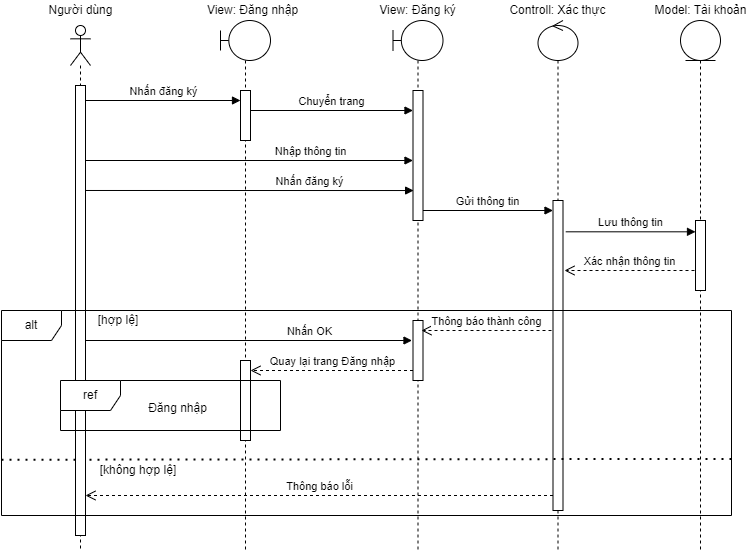
\includegraphics[width=14.5cm,height=11cm]{Images/sequence/sequence_register.png}
  \caption[Sơ đồ tuần tự chức năng đăng ký tài khoản]{\bfseries \fontsize{12pt}{0pt}
  \selectfont Sơ đồ tuần tự chức năng đăng ký tài khoản}
  \label{sequence_register} %đặt tên cho ảnh
\end{figure}
Sơ đồ tuần tự trên mô tả chi tiết quá trình người dùng đăng ký tài khoản trên hệ thống. Người dùng sẽ gửi yêu cầu đăng ký, yêu cầu sẽ được xử lý
bởi Control, nếu có lỗi phát sinh sẽ hiển thị lên màn hình và yêu cầu người dùng nhập lại. Nếu việc đăng ký thành công, Control sẽ gửi thông báo 
thành công và chuyển sang trang đăng nhập.  

\subsubsection{Sơ đồ tuần tự chức năng đăng nhập/đăng xuất}
\begin{figure}[H]
  \centering
  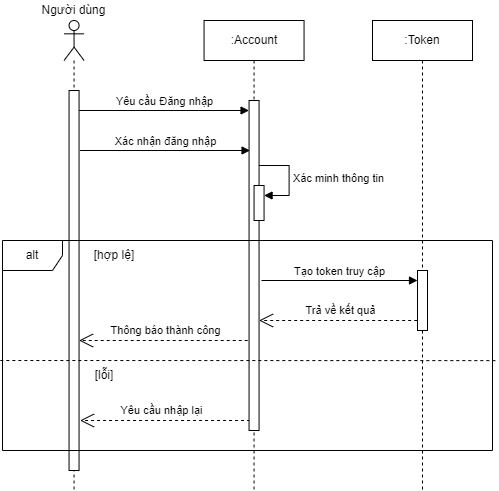
\includegraphics[width=14.5cm,height=9.5cm]{Images/sequence/sequence_login.png}
  \caption[Sơ đồ tuần tự chức năng đăng nhập]{\bfseries \fontsize{12pt}{0pt}
  \selectfont Sơ đồ tuần tự chức năng đăng nhập}
  \label{sequence_login} %đặt tên cho ảnh
\end{figure}
Sơ đồ tuần tự trên mô tả chi tiết quá trình người dùng đăng nhập trên hệ thống. Người dùng sẽ gửi yêu cầu đăng nhập, yêu cầu sẽ được xử lý
bởi Control, nếu có lỗi phát sinh sẽ hiển thị lên màn hình và yêu cầu người dùng nhập lại. Nếu việc đăng ký thành công, Control sẽ gửi thông báo 
thành công và chuyển sang trang chủ. 
\begin{figure}[H]
  \centering
  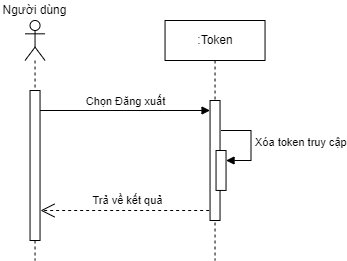
\includegraphics[width=14cm,height=8.5cm]{Images/sequence/sequence_logout.png}
  \caption[Sơ đồ tuần tự chức năng đăng xuất]{\bfseries \fontsize{12pt}{0pt}
  \selectfont Sơ đồ tuần tự chức năng đăng xuất}
  \label{sequence_logout} %đặt tên cho ảnh
\end{figure}
Sơ đồ tuần tự trên mô tả chi tiết quá trình người dùng đăng xuất khỏi hệ thống. Người dùng sẽ gửi yêu cầu đăng xuất, yêu cầu sẽ được xử lý
bởi Control. Nếu việc đăng xuất thành công, Control sẽ gửi thông báo 
thành công và chuyển sang trang đăng nhập. 

\subsubsection{Sơ đồ tuần tự chức năng quên mật khẩu}
\begin{figure}[H]
  \centering
  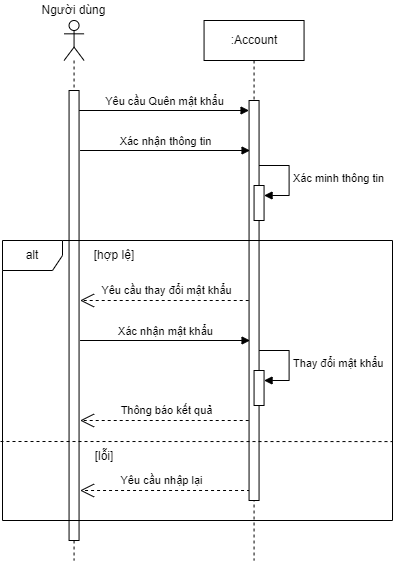
\includegraphics[width=15cm,height=15.5cm]{Images/sequence/sequence_forgot_password.png}
  \caption[Sơ đồ tuần tự chức năng quên mật khẩu]{\bfseries \fontsize{12pt}{0pt}
  \selectfont Sơ đồ tuần tự chức năng quên mật khẩu}
  \label{sequence_forgot_pass} %đặt tên cho ảnh
\end{figure}
Sơ đồ tuần tự trên mô tả chi tiết quá trình người dùng thay đổi mật khẩu trên hệ thống. Người dùng sẽ gửi nhập email đã đăng ký tài khoản, gửi yêu cầu
lấy lại mật khẩu. Yêu cầu sẽ được xử lý bởi Control, nếu có lỗi phát sinh sẽ hiển thị lên màn hình và yêu cầu người dùng nhập lại. Control sẽ gửi một mã xác thực
đến email, người dùng sẽ nhập mã xác thực và thay đổi mật khẩu mới. Nếu việc đăng ký thành công,
Control sẽ gửi thông báo thành công và chuyển sang đăng nhập.

\subsubsection{Sơ đồ tuần tự chức năng quản lý tài khoản cá nhân}
\begin{figure}[H]
  \centering
  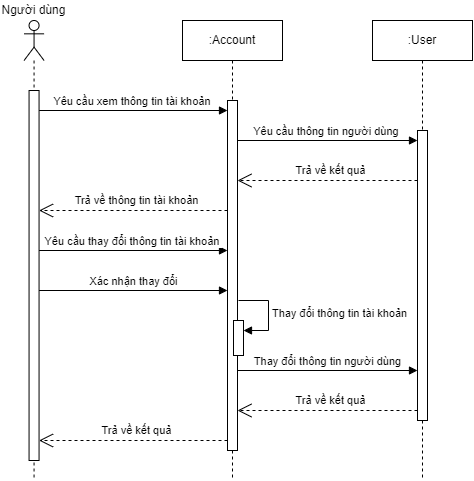
\includegraphics[width=14cm,height=10.5cm]{Images/sequence/sequence_manage_info.png}
  \caption[Sơ đồ tuần tự chức năng quản lý tài khoản cá nhân]{\bfseries \fontsize{12pt}{0pt}
  \selectfont Sơ đồ tuần tự chức năng quản lý tài khoản cá nhân}
  \label{sequence_account} %đặt tên cho ảnh
\end{figure}
Sơ đồ tuần tự trên mô tả chi tiết quá trình người dùng xem và thay đổi thông tin tài khoản trên hệ thống. Người dùng thay đổi thông tin và gửi yêu cầu, 
yêu cầu sẽ được xử lý bởi Control, nếu có lỗi phát sinh sẽ hiển thị lên màn hình và yêu cầu người dùng nhập lại. Nếu việc thay đổi thành công, Control sẽ gửi thông báo 
thành công.  

\subsubsection{Sơ đồ tuần tự chức năng quản lý dữ liệu đo}
\begin{figure}[H]
  \centering
  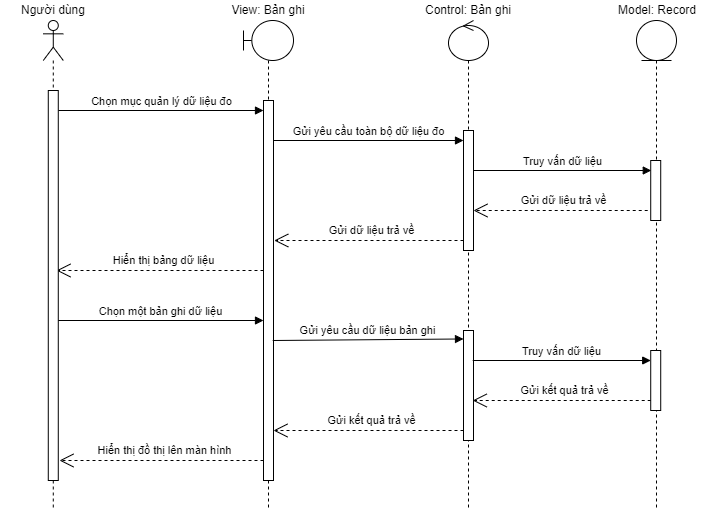
\includegraphics[width=14cm,height=10cm]{Images/sequence/sequence_manage_record.png}
  \caption[Sơ đồ tuần tự chức năng xem dữ liệu đo]{\bfseries \fontsize{12pt}{0pt}
  \selectfont Sơ đồ tuần tự chức năng xem dữ liệu đo}
  \label{sequence_manage_record} %đặt tên cho ảnh
\end{figure}
Sơ đồ tuần tự trên mô tả chi tiết quá trình người dùng xem dữ liệu đo từ thiết bị trên hệ thống. Người dùng chọn mở giao diện quản lý dữ liệu đo, 
API sẽ được xử lý bởi Control, hiện danh sách các bản ghi dữ liệu đo cho người dùng, người dùng có thể chọn một bản ghi dữ liệu và xem đồ thị biểu diễn
của nó. 

\begin{figure}[H]
  \centering
  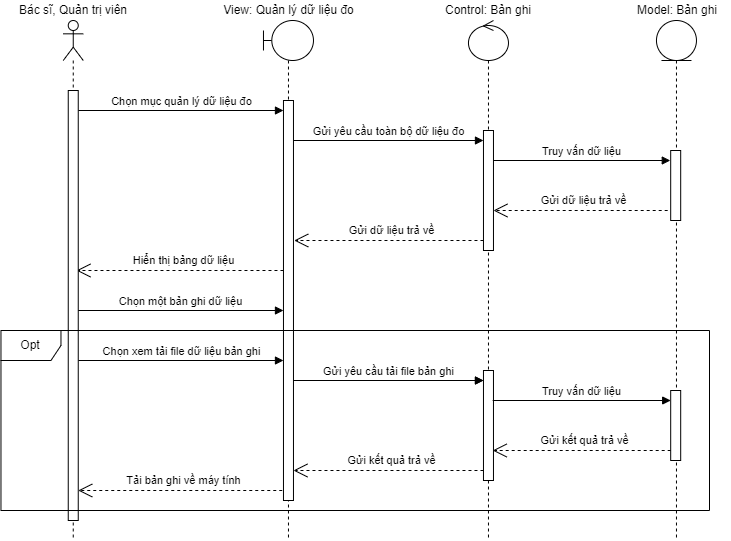
\includegraphics[width=14cm,height=10cm]{Images/sequence/sequence_download_records.png}
  \caption[Sơ đồ tuần tự chức năng tải dữ liệu đo]{\bfseries \fontsize{12pt}{0pt}
  \selectfont Sơ đồ tuần tự chức năng tải dữ liệu đo}
  \label{sequence_download_record} %đặt tên cho ảnh
\end{figure}
Nếu bác sĩ, quản trị viên muốn tải dữ liệu bản nghĩ, bác sĩ và quản trị viên gửi yêu cầu thay đổi, yêu cầu sẽ được xử lý bởi Control, 
nếu có lỗi phát sinh sẽ hiển thị lên màn hình, nếu thay đổi thành công Control sẽ gửi file về máy tính. 
\subsubsection{Sơ đồ tuần tự chức năng quản lý dịch vụ nhắn tin}
\begin{figure}[H]
  \centering
  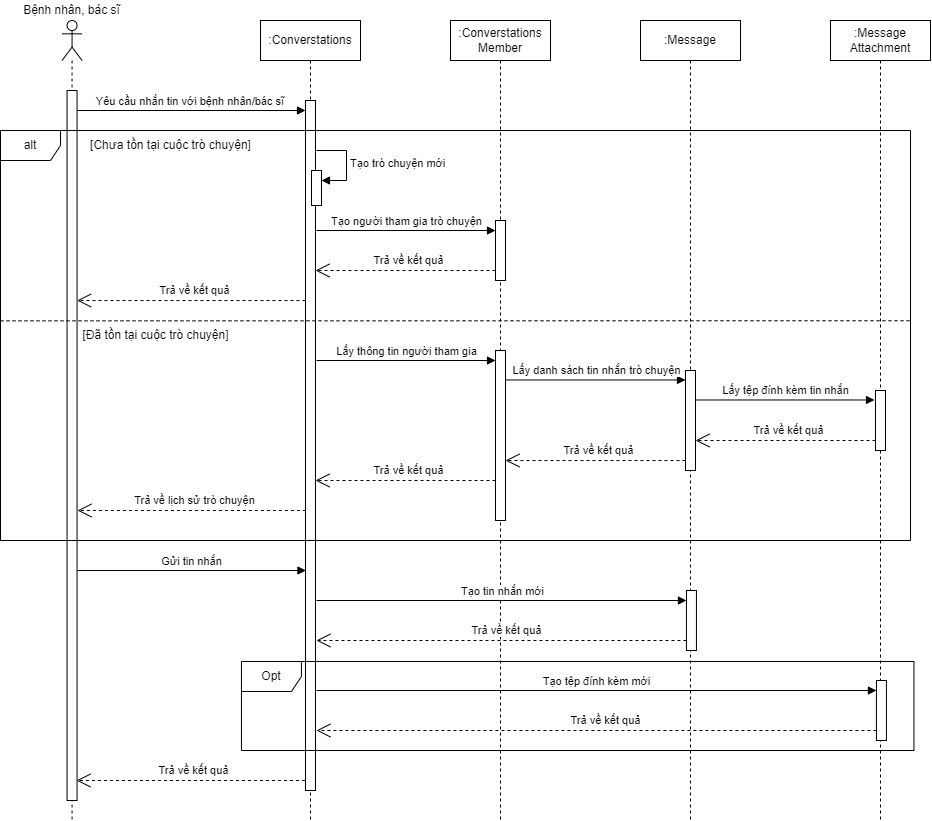
\includegraphics[width=14cm,height=10cm]{Images/sequence/sequence_chat.png}
  \caption[Sơ đồ tuần tự chức năng quản lý dịch vụ nhắn tin]{\bfseries \fontsize{12pt}{0pt}
  \selectfont Sơ đồ tuần tự chức năng quản lý dịch vụ nhắn tin}
  \label{sequence_chat} %đặt tên cho ảnh
\end{figure}
Sơ đồ tuần tự trên mô tả chi tiết quá trình người dùng xem và gửi tin nhắn giữa bệnh nhân và bác sĩ trên hệ thống. Người dùng chọn mở giao diện nhắn tin, 
chọn người mà mình muốn xem/gửi tin nhắn. Khi đó API sẽ được xử lý bởi Control, hiện lịch sử đoạn hội thoại. nếu người dùng gửi tin nhắn, yêu cầu sẽ được 
xử lý bởi Control gửi tin nhắn đến đối phương và lưu vào cơ sở dữ liệu.

\subsubsection{Sơ đồ tuần tự chức năng tư vấn từ trợ lý ảo}
\begin{figure}[H]
  \centering
  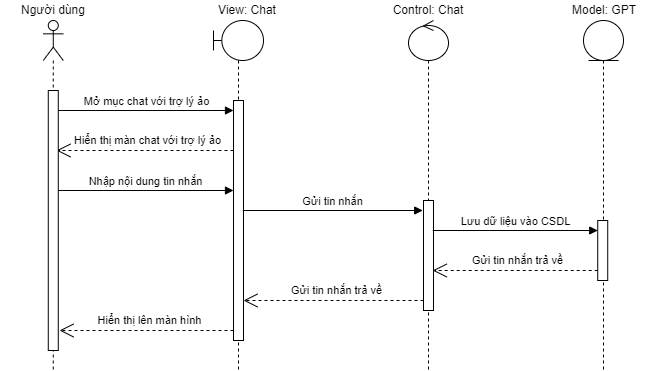
\includegraphics[width=14cm,height=9.5cm]{Images/sequence/sequence_chat_ai.png}
  \caption[Sơ đồ tuần tự chức năng tư vấn từ trợ lý ảo]{\bfseries \fontsize{12pt}{0pt}
  \selectfont Sơ đồ tuần tự chức năng tư vấn từ trợ lý ảo}
  \label{sequence_chat_ai} %đặt tên cho ảnh
\end{figure}
Sơ đồ tuần tự trên mô tả chi tiết quá trình người dùng xem và gửi tin nhắn với trợ lý ảo trên hệ thống. Người dùng chọn mở giao diện nhắn tin với trợ lý ảo, 
khi người dùng gửi tin nhắn đến trợ lý ảo, API sẽ được xử lý bởi Control gửi đến trợ lý ảo và phản hồi lại câu trả lời từ trợ lý ảo.


\subsubsection{Sơ đồ tuần tự chức năng quản lý bệnh nhân}
\begin{figure}[H]
  \centering
  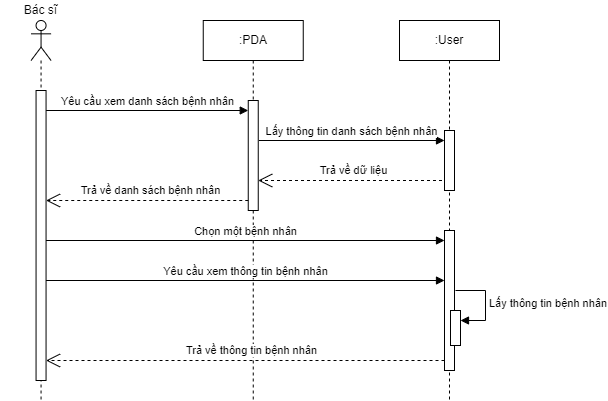
\includegraphics[width=14cm,height=11cm]{Images/sequence/sequence_manage_patient.png}
  \caption[Sơ đồ tuần tự chức năng quản lý bệnh nhân]{\bfseries \fontsize{12pt}{0pt}
  \selectfont Sơ đồ tuần tự chức năng quản lý bệnh nhân}
  \label{sequence_manage_patient} %đặt tên cho ảnh
\end{figure}
Sơ đồ tuần tự trên mô tả chi tiết quá trình bác sĩ xem, sửa, xóa với danh sách bệnh nhân trên hệ thống. Bác sĩ chọn mở giao diện quản lý bệnh nhân, 
API sẽ được xử lý bởi Control, hiện danh sách bệnh nhân, bác sĩ có thể chọn một bệnh nhân và xem thông tin của họ. 
\begin{figure}[H]
  \centering
  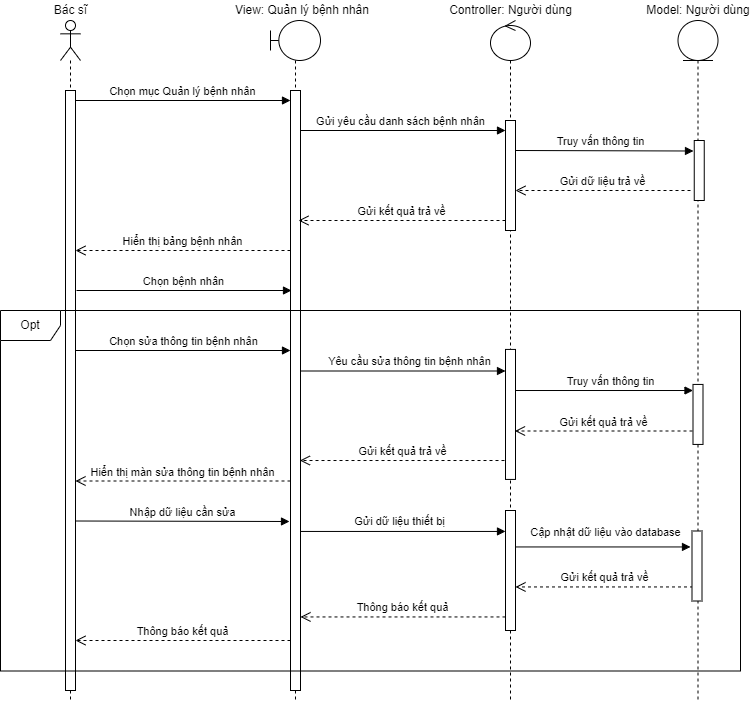
\includegraphics[width=14cm,height=13cm]{Images/sequence/sequence_manage_edit_patient.png}
  \caption[Sơ đồ tuần tự chức năng sửa thông tin bệnh nhân]{\bfseries \fontsize{12pt}{0pt}
  \selectfont Sơ đồ tuần tự chức năng sửa thông tin bệnh nhân}
  \label{sequence_manage_edit_patient} %đặt tên cho ảnh
\end{figure}
Nếu bác sĩ muốn chỉnh sửa thông tin bệnh nhân, bác sĩ nhập các thông tin cần sửa và gửi yêu cầu thay đổi, yêu cầu sẽ được xử lý bởi Control, 
nếu có lỗi phát sinh sẽ hiển thị lên màn hình, nếu thay đổi thành công Control sẽ gửi thông báo thành công. 
\begin{figure}[H]
  \centering
  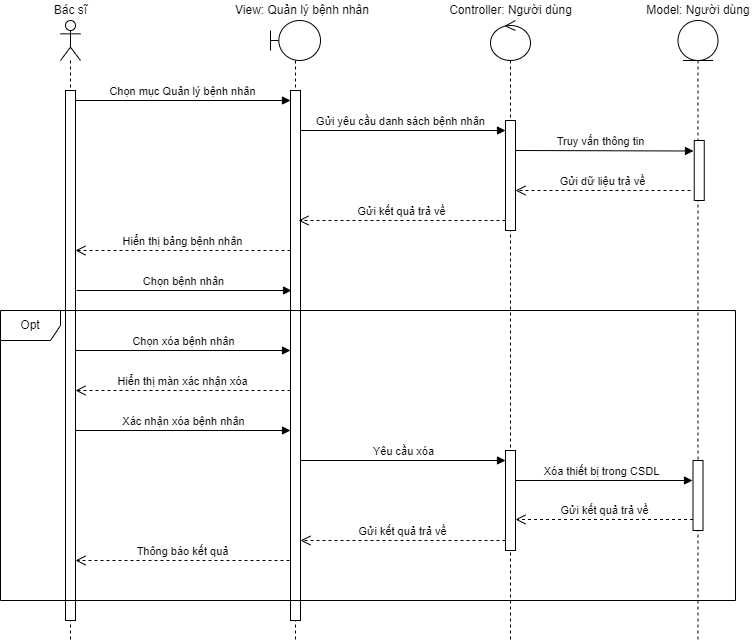
\includegraphics[width=14cm,height=12cm]{Images/sequence/sequence_manage_delete_patient.png}
  \caption[Sơ đồ tuần tự chức năng xóa bệnh nhân]{\bfseries \fontsize{12pt}{0pt}
  \selectfont Sơ đồ tuần tự chức năng xóa bệnh nhân}
  \label{sequence_manage_delete_patient} %đặt tên cho ảnh
\end{figure}
Nếu bác sĩ yêu cầu xóa bệnh nhân, Control sẽ xử lý xóa bệnh nhân ở cơ sở dữ liệu và trả về thông báo cho bác sĩ.  


\subsubsection{Sơ đồ tuần tự chức năng quản lý thiết bị}
\begin{figure}[H]
  \centering
  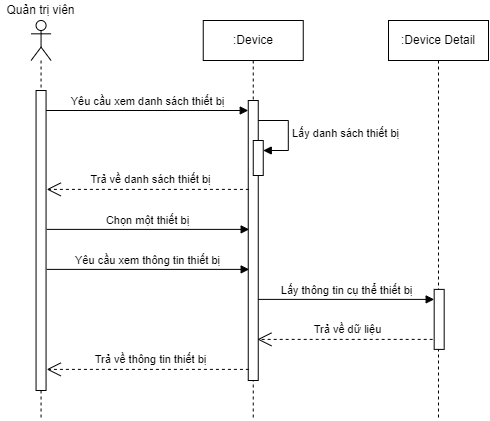
\includegraphics[width=14cm,height=11cm]{Images/sequence/sequence_manage_device.png}
  \caption[Sơ đồ tuần tự chức năng quản lý thiết bị]{\bfseries \fontsize{12pt}{0pt}
  \selectfont Sơ đồ tuần tự chức năng quản lý thiết bị}
  \label{sequence_manage_device} %đặt tên cho ảnh
\end{figure}
Sơ đồ tuần tự trên mô tả chi tiết quá trình quản trị viên xem, tạo, sửa, xóa với danh sách thiết bị trên hệ thống. Quản trị viên chọn mở giao diện quản lý thiết bị, 
API sẽ được xử lý bởi Control, hiện danh sách thiết bị, quản trị viên có thể chọn một thiết bị và xem thông tin của họ. 
\begin{figure}[H]
  \centering
  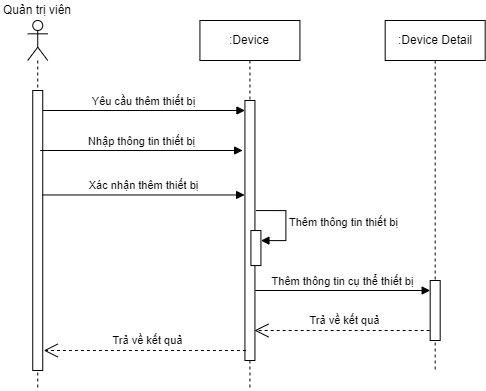
\includegraphics[width=14cm,height=11cm]{Images/sequence/sequence_manage_add_device.png}
  \caption[Sơ đồ tuần tự chức năng thêm thiết bị]{\bfseries \fontsize{12pt}{0pt}
  \selectfont Sơ đồ tuần tự chức năng thêm thiết bị}
  \label{sequence_manage_add_device} %đặt tên cho ảnh
\end{figure}
Nếu quản trị viên muốn tạo một thiết bị mới, quản trị viên nhập các thông tin và gửi yêu cầu tạo, yêu cầu sẽ được xử lý bởi Control, nếu có lỗi phát sinh sẽ hiển thị lên màn hình, nếu tạo thành công Control 
sẽ gửi thông báo thành công. 
\begin{figure}[H]
  \centering
  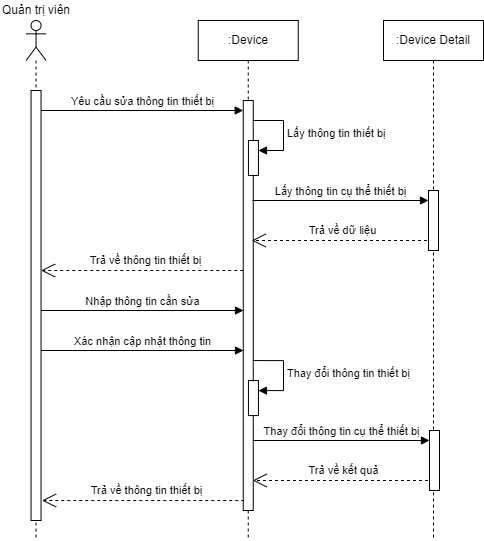
\includegraphics[width=14cm,height=13cm]{Images/sequence/sequence_manage_edit_device.png}
  \caption[Sơ đồ tuần tự chức năng sửa thông tin thiết bị]{\bfseries \fontsize{12pt}{0pt}
  \selectfont Sơ đồ tuần tự chức năng sửa thông tin thiết bị}
  \label{sequence_manage_edit_device} %đặt tên cho ảnh
\end{figure}
Nếu quản trị viên muốn chỉnh sửa thông tin thiết bị, quản trị viên nhập các thông tin cần sửa và gửi yêu cầu thay đổi, yêu cầu sẽ được xử lý
bởi Control, nếu có lỗi phát sinh sẽ hiển thị lên màn hình, nếu thay đổi thành công Control sẽ gửi thông báo thành công. 
\begin{figure}[H]
  \centering
  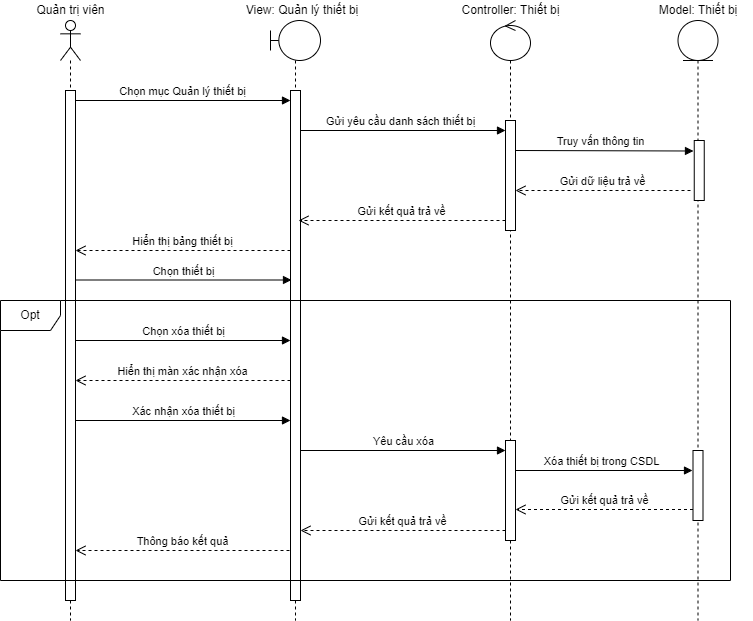
\includegraphics[width=14cm,height=12cm]{Images/sequence/sequence_manage_delete_device.png}
  \caption[Sơ đồ tuần tự chức năng xóa thiết bị]{\bfseries \fontsize{12pt}{0pt}
  \selectfont Sơ đồ tuần tự chức năng xóa thiết bị}
  \label{sequence_manage_delete_device} %đặt tên cho ảnh
\end{figure}
Nếu quản trị viên yêu cầu xóa thiết bị, Control sẽ xử lý xóa thiết bị ở cơ sở dữ liệu và trả về thông báo cho quản trị viên.

\subsubsection{Sơ đồ tuần tự chức năng quản lý tài khoản người dùng}
\begin{figure}[H]
  \centering
  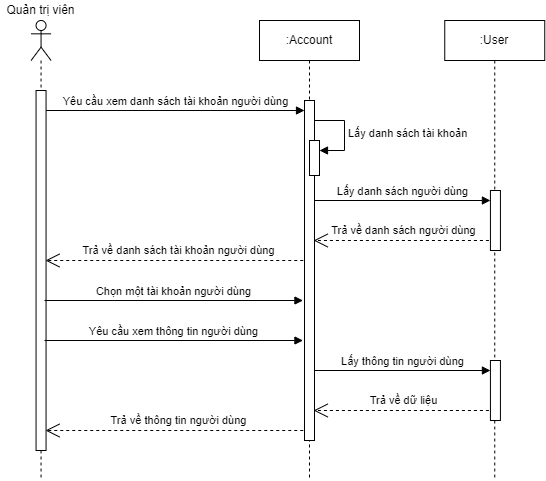
\includegraphics[width=14cm,height=11cm]{Images/sequence/sequence_manage_user.png}
  \caption[Sơ đồ tuần tự chức năng quản lý người dùng]{\bfseries \fontsize{12pt}{0pt}
  \selectfont Sơ đồ tuần tự chức năng quản lý người dùng}
  \label{sequence_manage_user} %đặt tên cho ảnh
\end{figure}
Sơ đồ tuần tự trên mô tả chi tiết quá trình quản trị viên xem, tạo, sửa, xóa với danh sách tài khoản người dùng trên hệ thống. Quản trị viên chọn mở giao diện
quản lý tài khoản người dùng, API sẽ được xử lý bởi Control, hiện danh sách thiết bị, quản trị viên có thể chọn một người dùng và xem thông tin của họ. 
\begin{figure}[H]
  \centering
  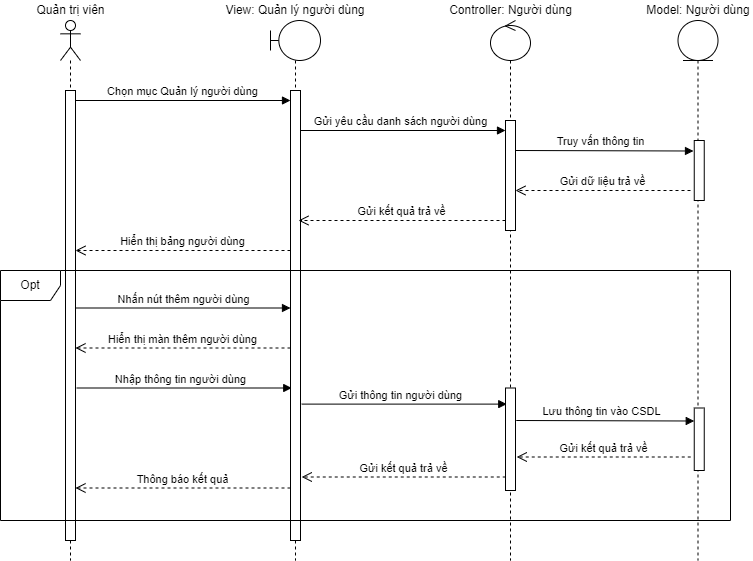
\includegraphics[width=14cm,height=11cm]{Images/sequence/sequence_manage_add_user.png}
  \caption[Sơ đồ tuần tự chức năng thêm người dùng]{\bfseries \fontsize{12pt}{0pt}
  \selectfont Sơ đồ tuần tự chức năng thêm người dùng}
  \label{sequence_manage_add_user} %đặt tên cho ảnh
\end{figure}
Nếu quản trị viên muốn thêm một người dùng mới, quản trị viên nhập các thông tin và gửi yêu cầu tạo, yêu cầu sẽ được xử lý bởi Control, nếu có lỗi phát sinh sẽ hiển thị lên màn hình,
nếu tạo thành công Control sẽ gửi thông báo thành công. 
\begin{figure}[H]
  \centering
  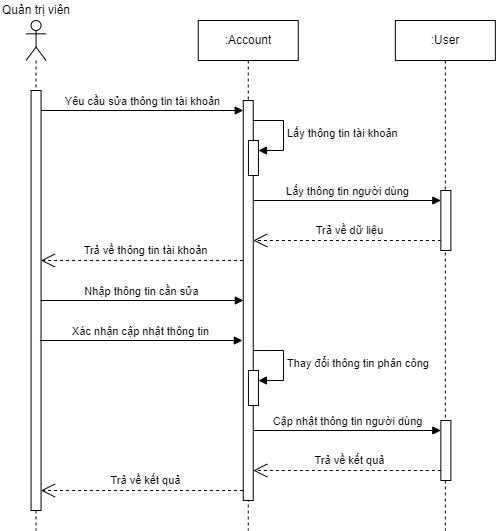
\includegraphics[width=14cm,height=13cm]{Images/sequence/sequence_manage_edit_user.png}
  \caption[Sơ đồ tuần tự chức năng sửa thông tin người dùng]{\bfseries \fontsize{12pt}{0pt}
  \selectfont Sơ đồ tuần tự chức năng sửa thông tin người dùng}
  \label{sequence_manage_edit_user} %đặt tên cho ảnh
\end{figure}
Nếu quản trị viên muốn chỉnh sửa thông tin người dùng, quản trị viên nhập các thông tin cần sửa và gửi yêu cầu thay đổi, yêu cầu sẽ được xử lý bởi Control, nếu có lỗi phát sinh sẽ hiển thị lên màn hình,
nếu thay đổi thành công Control sẽ gửi thông báo thành công. 
\begin{figure}[H]
  \centering
  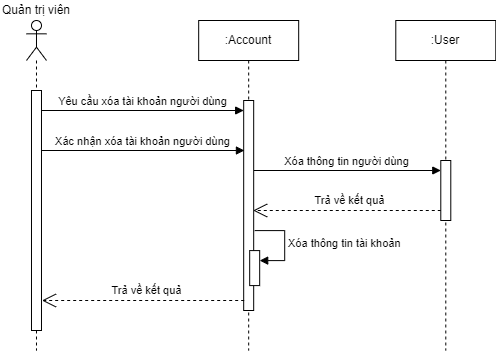
\includegraphics[width=14cm,height=12cm]{Images/sequence/sequence_manage_delete_user.png}
  \caption[Sơ đồ tuần tự chức năng xóa người dùng]{\bfseries \fontsize{12pt}{0pt}
  \selectfont Sơ đồ tuần tự chức năng xóa người dùng}
  \label{sequence_manage_delete_user} %đặt tên cho ảnh
\end{figure}
Nếu quản trị viên yêu cầu xóa tài khoản người dùng, Control sẽ xử lý xóa tài khoản ở cơ sở dữ liệu và trả về thông báo cho quản trị viên.
\begin{figure}[H]
  \centering
  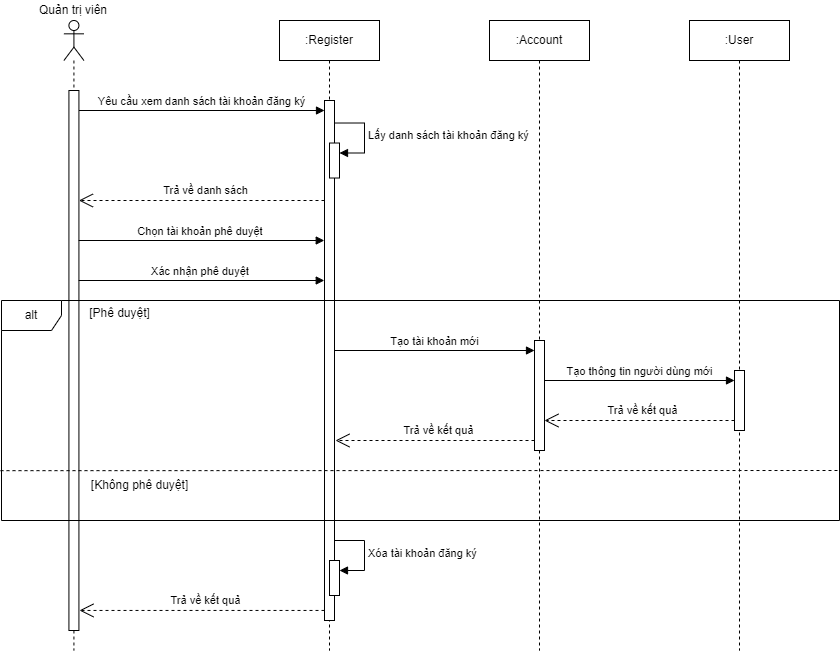
\includegraphics[width=14cm,height=13.5cm]{Images/sequence/sequence_manage_register.png}
  \caption[Sơ đồ tuần tự chức năng phê duyệt tài khoản người dùng]{\bfseries \fontsize{12pt}{0pt}
  \selectfont Sơ đồ tuần tự chức năng phê duyệt tài khoản người dùng}
  \label{sequence_manage_register} %đặt tên cho ảnh
\end{figure}
Nếu quản trị viên muốn phê duyệt tài khoản người dùng, quản trị sẽ chọn phê duyệt hoặc không phê duyệt, yêu cầu sẽ được xử lý bởi Control, nếu có lỗi phát sinh sẽ hiển thị lên màn hình,
nếu phê duyệt thành công Control sẽ gửi thông báo thành công. 

\subsection{Phân tích dữ liệu}

Tại phần này, chúng em sẽ tiến hành xác định và mô tả các thực thể cũng như
 thuộc tính quan trọng trong hệ thống. Việc này giúp chúng ta có cái
  nhìn tổng quan về các yếu tố chính cần được quản lý và lưu trữ
   trong cơ sở dữ liệu. Bằng cách làm điều này, chúng ta có thể
    xây dựng một mô hình dữ liệu cơ bản để hỗ trợ việc thiết kế và
     triển khai hệ thống một cách hiệu quả.

     Trước hết, chúng em sẽ xác định và mô tả các thực thể chính trong hệ
      thống. Thực thể là các đối tượng hoặc khái niệm quan
       trọng mà chúng ta cần theo dõi và quản lý. Sau đó, chúng ta sẽ xác
        định các thuộc tính liên quan đến mỗi thực thể, các thông tin cần
         được lưu trữ và quản lý.

\begin{table}[H]
  \caption{\bfseries \fontsize{12pt}{0pt}\selectfont Bảng thực thể và thuộc tính}
  \centering
  \begin{tabularx}{0.9\textwidth}{|c|X|}
    \hline
    \textbf{Thực thể} & \textbf{Thuộc tính} \\
    \hline
    Người dùng & 
    ID người dùng, ID tài khoản, Tên người dùng, Email, Mật khẩu, Ngày sinh, Giới tính, Số điện thoại, Quyền, Thông tin người dùng \\
    \hline
    Token đăng nhập &
    ID token, ID tài khoản, Token truy cập, Token làm mới \\
    \hline
    Thiết bị & 
    ID thiết bị, ID người dùng thiết bị, ID bác sĩ theo dõi, Tên thiết bị, Loại thiết bị, Thông tin thiết bị, Trạng thái thiết bị, Ngày bắt đầu sử dụng\\
    \hline
    Các tần số đo được của thiết bị &
    ID tần số, ID thiết bị, Tên loại tần số, Thông tin, Giá trị đo được \\
    \hline
    Bản ghi dữ liệu & 
    ID bản ghi dữ liệu, ID người dùng, ID thiết bị, Loại bản ghi, Đường dẫn lưu trữ dữ liệu, Thời gian bắt đầu đo, Thời gian kết thúc đo \\
    \hline
    Thông tin hội thoại &
    ID hội thoại, Tên hội thoại, Loại hội thoại, Đường dẫn avatar hội thoại \\
    \hline
    Thành viên tham gia hội thoại &
    ID hội thoại, ID người dùng tham gia, Trạng thái thông báo (Có thông báo, Không thông báo), Tác vụ (người tạo đoạn hội thoại, thành viên trong đoạn hội thoại), Trạng thái đã xem\\
    \hline
    Tin nhắn & 
    ID tin nhắn, ID hội thoại, ID người gửi, Các tệp đính kèm, Tin nhắn hệ thống, Ghim (tin nhắn được ghim, không được ghim), Thời gian ghim tin nhắn, Các lượt thả cảm xúc \\
    \hline
    Tệp đính kèm &
    ID tệp đính kèm, ID tin nhắn, ID hội thoại, Đường dẫn nội dung, Tên tệp, Kích thước tệp, Đường dẫn thumbnail, Loại đính kèm (hình ảnh, video, tệp tin) \\
    \hline 
    Phân công bệnh nhân - bác sĩ & 
    ID phân công, ID bệnh nhân, ID bác sĩ, Ngày bắt đầu, Ngày kết thúc \\
    \hline
    Danh mục tin tức &
    ID danh mục tin tức, Tên danh mục tin tức, Mô tả danh mục tin tức \\
    \hline
    Tin tức &
    ID tin tức, Tiêu đề, Nội dung, ID danh mục tin tức, Tác giả, Đường dẫn, Đường dẫn hình ảnh \\
    \hline
  \end{tabularx}

  
\end{table}
Sau khi hoàn thành được bảng thực thể và thuộc tính, chúng em xác định được mô hình thực thể liên kết như sau:

\begin{figure}[H]
  \centering
  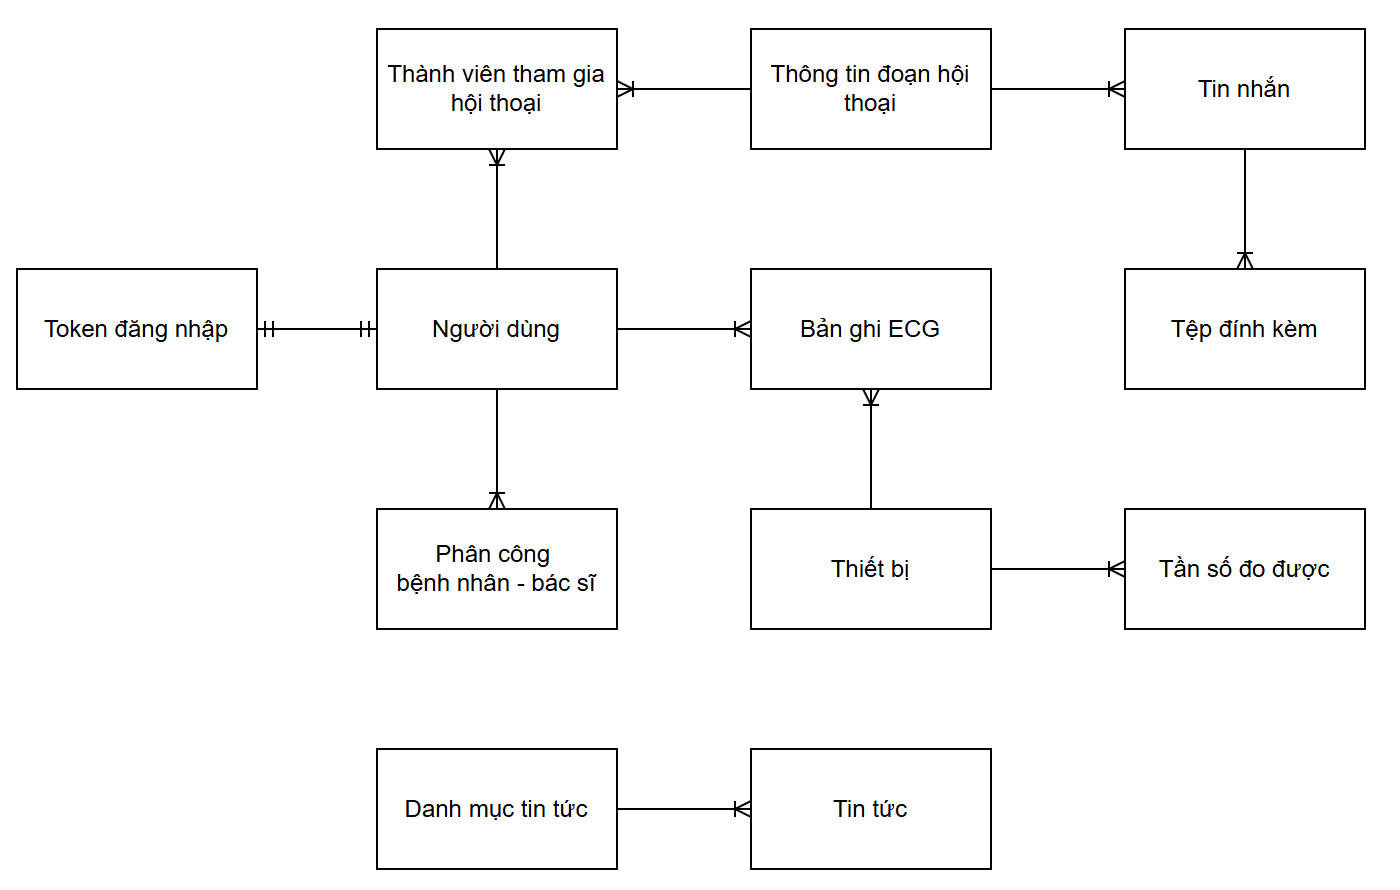
\includegraphics[width=15cm,height=10cm]{Images/system/fmECG_connection_entity.png}
  \caption[Mô hình thực thể liên kết]{\bfseries \fontsize{12pt}{0pt}
  \selectfont Mô hình thực thể liên kết}
  \label{ttlk} %đặt tên cho ảnh
\end{figure}

\subsection{Mô hình quan hệ}
Dựa trên phần mô tả các thực thể, chúng em sẽ chuyển mô hình thực thể liên kết sang mô hình quan hệ như sau:

\begin{itemize}
  \item Người dùng (\textbf{ID người dùng}, ID tài khoản, Tên người dùng, Email, Mật khẩu, Ngày sinh, Giới tính, Số điện thoại, Quyền, Thông tin người dùng)
  \item Token đăng nhập (\textbf{ID token}, ID tài khoản, Token truy cập, Token làm mới)
  \item Thiết bị (\textbf{ID thiết bị}, ID người dùng thiết bị, ID bác sĩ theo dõi, Tên thiết bị, Loại thiết bị, Thông tin thiết bị, Trạng thái thiết bị, Ngày bắt đầu sử dụng)
  \item Bản ghi dữ liệu (\textbf{ID bản ghi dữ liệu}, ID người dùng, ID thiết bị, Loại bản ghi, Đường dẫn lưu trữ dữ liệu, Thời gian bắt đầu đo, Thời gian kết thúc đo)
  \item Thông tin hội thoại (\textbf{ID hội thoại}, Tên hội thoại, Loại hội thoại, Đường dẫn avatar hội thoại)
  \item Thành viên tham gia hội thoại (\textbf{ID}, ID hội thoại, ID người dùng tham gia, Trạng thái thông báo, Tác vụ, Trạng thái đã xem)
  \item Tin nhắn (\textbf{ID tin nhắn}, ID hội thoại, ID người gửi, Các tệp đính kèm, Tin nhắn hệ thống, Ghim, Thời gian ghim tin nhắn, Các lượt thả cảm xúc)
  \item Tệp đính kèm (\textbf{ID tệp đính kèm}, ID tin nhắn, ID hội thoại, Đường dẫn nội dung, Tên tệp, Kích thước tệp, Đường dẫn thumbnail, Loại đính kèm)
  \item Phân công bệnh nhân - bác sĩ (\textbf{ID phân công}, ID bệnh nhân, ID bác sĩ, Ngày bắt đầu)
  \item Danh mục tin tức (\textbf{ID danh mục tin tức}, Tên danh mục tin tức, Mô tả danh mục tin tức)
  \item Tin tức (\textbf{ID tin tức}, Tiêu đề, Nội dung, ID danh mục tin tức, Tác giả, Đường dẫn, Đường dẫn hình ảnh)
\end{itemize}


\subsection{Chuẩn hoá 3NF}
Các bảng đã được thiết kế theo nguyên tắc chuẩn hoá 3NF, vì không có thuộc tính lặp lại và các thuộc tính không phụ thuộc vào một tập hợp con của khóa chính.

\subsubsection{Chuẩn hoá bảng Người dùng}

\begin{table}[H]
  \caption{\bfseries \fontsize{12pt}{0pt}\selectfont Bảng chuẩn hoá bảng Người dùng}
  \centering
  \begin{tabularx}{0.9\textwidth}{|X|X|}
    \hline
    \textbf{Danh sách thuộc tính} & ID người dùng, ID tài khoản, Tên người dùng, Email, Mật khẩu, Ngày sinh, Giới tính, Số điện thoại, Quyền, Thông tin người dùng \\
    \hline
    \textbf{Quy tắc nghiệp vụ} & \textbf{Phụ thuộc hàm} \\
    \hline
    Mỗi người dùng có một ID riêng, có duy nhất mật khẩu, email, tên, ngày sinh, số điện thoại, quyền,
    giới tính, thông tin & \parbox[t]{\linewidth}{$\text{ID người dùng} \rightarrow$ mật khẩu, email, tên, ngày sinh, số điện thoại, quyền, thông tin} \\
    \hline
    \multicolumn{2}{|X|}{$\Rightarrow \text{Khoá chính của bảng: ID người dùng}$} \\
    \multicolumn{2}{|X|}{$\Rightarrow \text{Bảng Người dùng đã ở 3NF}$} \\
    \hline
  \end{tabularx}
\end{table}

\subsubsection{Chuẩn hoá bảng Token đăng nhập}

\begin{table}[H]
  \caption{\bfseries \fontsize{12pt}{0pt}\selectfont Bảng chuẩn hoá bảng Token đăng nhập}
  \centering
  \begin{tabularx}{0.9\textwidth}{|X|X|}
    \hline
    \textbf{Danh sách thuộc tính} & ID token, ID tài khoản, Token truy cập, Token làm mới \\
    \hline
    \textbf{Quy tắc nghiệp vụ} & \textbf{Phụ thuộc hàm} \\
    \hline
    Mỗi người dùng có một ID token riêng, có duy nhất ID tài khoản, token truy cập và token làm mới 
    & \parbox[t]{\linewidth}{$\text{ID token} \rightarrow$ ID tài khoản, Token truy cập, Token làm mới} \\
    \hline
    \multicolumn{2}{|X|}{$\Rightarrow \text{Khoá chính của bảng: ID token đăng nhập}$} \\
    \multicolumn{2}{|X|}{$\Rightarrow \text{Bảng Token  đã ở 3NF}$} \\
    \hline
  \end{tabularx}
\end{table}

\subsubsection{Chuẩn hoá bảng Thiết bị}

\begin{table}[H]
  \caption{\bfseries \fontsize{12pt}{0pt}\selectfont Bảng chuẩn hoá bảng Thiết bị}
  \centering
  \begin{tabularx}{0.9\textwidth}{|X|X|}
    \hline
    \textbf{Danh sách thuộc tính} & ID thiết bị, ID người dùng thiết bị, ID bác sĩ theo dõi, Tên thiết bị, 
    Loại thiết bị, Thông tin thiết bị, Trạng thái thiết bị, Ngày bắt đầu sử dụng \\
    \hline
    \textbf{Quy tắc nghiệp vụ} & \textbf{Phụ thuộc hàm} \\
    \hline
    Mỗi thiết bị khi được sử dụng sẽ có một ID thiết bị riêng, có duy nhất tên thiết bị, loại thiết bị, thông tin thiết bị.
    ID người dùng thiết bị, ID bác sĩ theo dõi, trạng thái thiết bị, ngày bắt đầu sử dụng
    & \parbox[t]{\linewidth}{$\text{ID thiết bị} \rightarrow$ ID người dùng thiết bị, ID bác sĩ theo dõi, Tên thiết bị, 
    Loại thiết bị, Thông tin thiết bị, Trạng thái thiết bị, Ngày bắt đầu sử dụng} \\
    \hline
    \multicolumn{2}{|X|}{$\Rightarrow \text{Khoá chính của bảng: ID thiết bị}$} \\
    \multicolumn{2}{|X|}{$\Rightarrow \text{Bảng Thiết bị đã ở 3NF}$} \\
    \hline
  \end{tabularx}
\end{table}

\subsubsection{Chuẩn hoá bảng Bản ghi dữ liệu}

\begin{table}[H]
  \caption{\bfseries \fontsize{12pt}{0pt}\selectfont Bảng chuẩn hoá bảng Bản ghi dữ liệu}
  \centering
  \begin{tabularx}{0.9\textwidth}{|X|X|}
    \hline
    \textbf{Danh sách thuộc tính} & ID bản ghi dữ liệu, ID người dùng, ID thiết bị, Loại bản ghi, 
    Đường dẫn lưu trữ dữ liệu, Thời gian bắt đầu đo, Thời gian kết thúc đo \\
    \hline
    \textbf{Quy tắc nghiệp vụ} & \textbf{Phụ thuộc hàm} \\
    \hline
    Mỗi bản ghi có một ID bản ghi dữ liệu riêng, có duy nhất ID người dùng, ID thiết bị, Loại bản ghi, 
    Đường dẫn lưu trữ dữ liệu, Thời gian bắt đầu đo, Thời gian kết thúc đo
    & \parbox[t]{\linewidth}{$\text{ID bản ghi dữ liệu} \rightarrow$ ID người dùng, ID thiết bị, Loại bản ghi, 
    Đường dẫn lưu trữ dữ liệu, Thời gian bắt đầu đo, Thời gian kết thúc đo} \\
    \hline
    \multicolumn{2}{|X|}{$\Rightarrow \text{Khoá chính của bảng: ID bản ghi dữ liệu}$} \\
    \multicolumn{2}{|X|}{$\Rightarrow \text{Bảng Bản ghi dữ liệu đã ở 3NF}$} \\
    \hline
  \end{tabularx}
\end{table}

\subsubsection{Chuẩn hoá bảng Thông tin hội thoại}

\begin{table}[H]
  \caption{\bfseries \fontsize{12pt}{0pt}\selectfont Bảng chuẩn hoá bảng Thông tin hội thoại}
  \centering
  \begin{tabularx}{0.9\textwidth}{|X|X|}
    \hline
    \textbf{Danh sách thuộc tính} & ID hội thoại, Tên hội thoại, 
    Loại hội thoại, Đường dẫn avatar hội thoại \\
    \hline
    \textbf{Quy tắc nghiệp vụ} & \textbf{Phụ thuộc hàm} \\
    \hline
    Mỗi hội thoại có một ID hội thoại riêng, có duy nhất tên hội thoại, 
    loại hội thoại, đường dẫn avatar hội thoại
    & \parbox[t]{\linewidth}{$\text{ID hội thoại} \rightarrow$ Tên hội thoại, 
    Loại hội thoại, Đường dẫn avatar hội thoại} \\
    \hline
    \multicolumn{2}{|X|}{$\Rightarrow \text{Khoá chính của bảng: ID hội thoại}$} \\
    \multicolumn{2}{|X|}{$\Rightarrow \text{Bảng Thông tin hội thoại đã ở 3NF}$} \\
    \hline
  \end{tabularx}
\end{table}

\subsubsection{Chuẩn hoá bảng Thành viên tham gia hội thoại}

\begin{table}[H]
  \caption{\bfseries \fontsize{12pt}{0pt}\selectfont Bảng chuẩn hoá bảng Thành viên tham gia hội thoại}
  \centering
  \begin{tabularx}{0.9\textwidth}{|X|X|}
    \hline
    \textbf{Danh sách thuộc tính} & ID, ID hội thoại, ID người dùng tham gia,
    Trạng thái thông báo, Tác vụ, Trạng thái đã xem \\
    \hline
    \textbf{Quy tắc nghiệp vụ} & \textbf{Phụ thuộc hàm} \\
    \hline
    Mỗi hội thoại có nhiều ID người dùng tham gia, mỗi người dùng có duy nhất trạng thái thông báo,
    tác vụ, trạng thái đã xem trong một hội thoại
    & \parbox[t]{\linewidth}{$\text{ID} \rightarrow$ ID hội thoại, ID người dùng tham gia,
    Trạng thái thông báo, Tác vụ, Trạng thái đã xem} \\
    \hline
    \multicolumn{2}{|X|}{$\Rightarrow \text{Khoá chính của bảng: ID}$} \\
    \multicolumn{2}{|X|}{$\Rightarrow \text{Bảng Thành viên tham gia hội thoại đã ở 3NF}$} \\
    \hline
  \end{tabularx}
\end{table}

\subsubsection{Chuẩn hoá bảng Tin nhắn}

\begin{table}[H]
  \caption{\bfseries \fontsize{12pt}{0pt}\selectfont Bảng chuẩn hoá bảng Tin nhắn}
  \centering
  \begin{tabularx}{0.9\textwidth}{|X|X|}
    \hline
    \textbf{Danh sách thuộc tính} & ID tin nhắn, ID hội thoại, ID người gửi, Các tệp đính kèm, 
    Tin nhắn hệ thống, Ghim, Thời gian ghim tin nhắn, Các lượt thả cảm xúc \\
    \hline
    \textbf{Quy tắc nghiệp vụ} & \textbf{Phụ thuộc hàm} \\
    \hline
    Mỗi tin nhắn có một ID tin nhắn riêng, thuộc một hội thoại, có duy nhất ID người gửi, các tệp đính kèm,
    tin nhắn hệ thống, ghim, thời gian ghim tin nhắn, các lượt thả cảm xúc
    & \parbox[t]{\linewidth}{$\text{ID tin nhắn} \rightarrow$ ID hội thoại, ID người gửi, các tệp đính kèm,
    tin nhắn hệ thống, ghim, thời gian ghim tin nhắn, các lượt thả cảm xúc} \\
    \hline
    \multicolumn{2}{|X|}{$\Rightarrow \text{Khoá chính của bảng: ID tin nhắn}$} \\
    \multicolumn{2}{|X|}{$\Rightarrow \text{Bảng Tin nhắn đã ở 3NF}$} \\
    \hline
  \end{tabularx}
\end{table}

\subsubsection{Chuẩn hoá bảng Tệp đính kèm}

\begin{table}[H]
  \caption{\bfseries \fontsize{12pt}{0pt}\selectfont Bảng chuẩn hoá bảng Tệp đính kèm}
  \centering
  \begin{tabularx}{0.9\textwidth}{|X|X|}
    \hline
    \textbf{Danh sách thuộc tính} & ID tệp đính kèm, ID tin nhắn, ID hội thoại, Đường dẫn nội
    dung, Tên tệp, Kích thước tệp, Đường dẫn thumbnail, Loại đính kèm \\
    \hline
    \textbf{Quy tắc nghiệp vụ} & \textbf{Phụ thuộc hàm} \\
    \hline
    Mỗi tệp đính kèm có một ID tệp đính kèm riêng, thuộc một tin nhắn trong một hội thoại, có duy nhất đường dẫn nội
    dung, tên tệp, kích thước tệp, đường dẫn thumbnail, loại đính kèm
    & \parbox[t]{\linewidth}{$\text{ID tệp đính kèm} \rightarrow$ ID tin nhắn, ID hội thoại, Đường dẫn nội
    dung, Tên tệp, Kích thước tệp, Đường dẫn thumbnail, Loại đính kèm} \\
    \hline
    \multicolumn{2}{|X|}{$\Rightarrow \text{Khoá chính của bảng: ID tệp đính kèm}$} \\
    \multicolumn{2}{|X|}{$\Rightarrow \text{Bảng Tệp đính kèm đã ở 3NF}$} \\
    \hline
  \end{tabularx}
\end{table}

\subsubsection{Chuẩn hoá bảng Phân công bệnh nhân - bác sĩ}

\begin{table}[H]
  \caption{\bfseries \fontsize{12pt}{0pt}\selectfont Bảng chuẩn hoá bảng Phân công bệnh nhân - bác sĩ}
  \centering
  \begin{tabularx}{0.9\textwidth}{|X|X|}
    \hline
    \textbf{Danh sách thuộc tính} & ID phân công, ID bệnh nhân, ID bác sĩ, Ngày bắt đầu \\
    \hline
    \textbf{Quy tắc nghiệp vụ} & \textbf{Phụ thuộc hàm} \\
    \hline
    Mỗi phân công bệnh nhân - bác sĩ có một ID phân công riêng, có duy nhất ID bệnh nhân, ID bác sĩ, ngày bắt đầu.
    Mỗi bệnh nhân thuộc một phân công duy nhất, còn mỗi bác sĩ có thể được giao nhiều phân công.
    & \parbox[t]{\linewidth}{$\text{ID phân công} \rightarrow$ ID bệnh nhân, ID bác sĩ, Ngày bắt đầu} \\
    \hline
    \multicolumn{2}{|X|}{$\Rightarrow \text{Khoá chính của bảng: ID phân công}$} \\
    \multicolumn{2}{|X|}{$\Rightarrow \text{Bảng Phân công bệnh nhân - bác sĩ đã ở 3NF}$} \\
    \hline
  \end{tabularx}
\end{table}

\subsubsection{Chuẩn hoá bảng Danh mục tin tức}

\begin{table}[H]
  \caption{\bfseries \fontsize{12pt}{0pt}\selectfont Bảng chuẩn hoá bảng Danh mục tin tức}
  \centering
  \begin{tabularx}{0.9\textwidth}{|X|X|}
    \hline
    \textbf{Danh sách thuộc tính} & ID danh mục tin tức, Tên danh mục tin tức, Mô tả danh mục tin tức \\
    \hline
    \textbf{Quy tắc nghiệp vụ} & \textbf{Phụ thuộc hàm} \\
    \hline
    Mỗi danh mục tin tức có một ID danh mục tin tức riêng, có duy nhất tên danh mục tin tức, mô tả danh mục tin tức
    & \parbox[t]{\linewidth}{$\text{ID danh mục tin tức} \rightarrow$ Tên danh mục tin tức, Mô tả danh mục tin tức} \\
    \hline
    \multicolumn{2}{|X|}{$\Rightarrow \text{Khoá chính của bảng: ID danh mục tin tức}$} \\
    \multicolumn{2}{|X|}{$\Rightarrow \text{Bảng Danh mục tin tức đã ở 3NF}$} \\
    \hline
  \end{tabularx}
\end{table}

\subsubsection{Chuẩn hoá bảng Tin tức}

\begin{table}[H]
  \caption{\bfseries \fontsize{12pt}{0pt}\selectfont Bảng chuẩn hoá bảng Tin tức}
  \centering
  \begin{tabularx}{0.9\textwidth}{|X|X|}
    \hline
    \textbf{Danh sách thuộc tính} & ID tin tức, Tiêu đề, Nội dung, ID danh mục tin tức, Tác giả, Đường dẫn,
    Đường dẫn hình ảnh \\
    \hline
    \textbf{Quy tắc nghiệp vụ} & \textbf{Phụ thuộc hàm} \\
    \hline
    Mỗi tin tức có một ID tin tức riêng, thuộc duy nhất một danh mục tin tức, có duy nhất tiêu đề, 
    nội dung, tác giả, đường dẫn, đường dẫn hình ảnh
    & \parbox[t]{\linewidth}{$\text{ID tin tức} \rightarrow$ Tiêu đề, Nội dung, ID danh mục tin tức, Tác giả, 
    Đường dẫn, Đường dẫn hình ảnh} \\
    \hline
    \multicolumn{2}{|X|}{$\Rightarrow \text{Khoá chính của bảng: ID tin tức}$} \\
    \multicolumn{2}{|X|}{$\Rightarrow \text{Bảng Tin tức đã ở 3NF}$} \\
    \hline
  \end{tabularx}
\end{table}

\subsection{Kết luận chương}

Trong chương này, chúng em đã thực hiện phân tích toàn diện về
 hệ thống cho đề tài , nhằm đáp ứng
  các mục tiêu và yêu cầu đã được đề xuất.

Chúng em đã xác định rõ ràng các khía cạnh quan trọng của hệ thống,
 tập trung vào việc thiết kế một hệ thống quản lý ECG hiệu quả,
  trực quan và có khả năng theo dõi sức khỏe tim mạch một cách
   chính xác. 


\newpage
